\documentclass[12pt,twoside,a4paper]{report}
\usepackage{etex}
% Select encoding of your inputs.
\usepackage[utf8]{inputenc}
\usepackage{imakeidx}

% Make latex understand and use the typographic
% rules of the language used in the document.
\usepackage[danish, english]{babel}

% Use the vector font Latin Modern which is going
% to be the default font in latex in the future.
\usepackage{lmodern}
% Use vector arrows in mathmode
\usepackage{esvect}

% Choose the font encoding
\usepackage[T1]{fontenc}

% load a colour package
\usepackage[table]{xcolor}
\definecolor{aaublue}{RGB}{33,26,82}% dark blue

% The standard graphics inclusion package
\definecolor{white}{RGB}{255,255,255} % define color white
\usepackage{graphicx}

% Set up how figure and table captions are displayed
\usepackage{caption}
\captionsetup{%
  font=footnotesize,% set font size to footnotesize
  labelfont=bf % bold label (e.g., Figure 3.2) font
}

% Enable row combination in tables
\usepackage{multirow}

% Make space between table lines and text
\renewcommand{\arraystretch}{1.5}

% Make the standard latex tables look so much better
\usepackage{array,booktabs}

% Enable the use of frames around, e.g., theorems
% The framed package is used in the example environment
\usepackage{framed}
\usepackage{colortbl}
\usepackage{longtable}

\usepackage{textcomp}

%%%%%%%%%%%%%%%%%%%%%%%%%%%%%%%%%%%%%%%%%%%%%%%%
% Mathematics
%%%%%%%%%%%%%%%%%%%%%%%%%%%%%%%%%%%%%%%%%%%%%%%%
% Defines new environments such as equation,
% align and split 
\usepackage{amsmath}
\usepackage{relsize}
% Adds new math symbols
\usepackage{amssymb}
% Use theorems in your document
% The ntheorem package is also used for the example environment
% When using thmmarks, amsmath must be an option as well. Otherwise \eqref doesn't work anymore.
\usepackage[framed,amsmath,thmmarks]{ntheorem}

%%%%%%%%%%%%%%%%%%%%%%%%%%%%%%%%%%%%%%%%%%%%%%%%
% Page Layout
%%%%%%%%%%%%%%%%%%%%%%%%%%%%%%%%%%%%%%%%%%%%%%%%
% Change margins, papersize, etc of the document
\usepackage[
  left=25mm,% left margin on an odd page %tidligere 25mm for baade right og left
  right=25mm,% right margin on an odd page
  top=35mm,
  ]{geometry}
  
% Modify how \chapter, \section, etc. look
% The titlesec package is very configureable
\usepackage{titlesec}
\makeatletter
\def\ttl@mkchap@i#1#2#3#4#5#6#7{%
    \ttl@assign\@tempskipa#3\relax\beforetitleunit
    \vspace{\@tempskipa}%<<<<<< REMOVE THE * AFTER \vspace
    \global\@afterindenttrue
    \ifcase#5 \global\@afterindentfalse\fi
    \ttl@assign\@tempskipb#4\relax\aftertitleunit
    \ttl@topmode{\@tempskipb}{%
        \ttl@select{#6}{#1}{#2}{#7}}%
    \ttl@finmarks  % Outside the box!
    \@ifundefined{ttlp@#6}{}{\ttlp@write{#6}}}
\makeatother

\titlespacing{\chapter}{0pt}{0pt}{10pt}
\titlespacing{\section}{0pt}{0pt}{-5pt}
\titlespacing{\subsection}{0pt}{8pt}{-5pt}
\titlespacing{\subsubsection}{0pt}{6pt}{-10pt}

\titleformat*{\section}{\normalfont\Large\bfseries}%\color{aaublue}}
\titleformat*{\subsection}{\normalfont\large\bfseries}%\color{aaublue}}
\titleformat*{\subsubsection}{\normalfont\normalsize\bfseries}%\color{aaublue}}
%\titleformat*{\paragraph}{\normalfont\normalsize\bfseries\color{aaublue}}
%\titleformat*{\subparagraph}{\normalfont\normalsize\bfseries\color{aaublue}}

%Formatting chapter headers. Predefined styles that can be used as option to the package: Sonny, Lenny, Glenn, Conny, Rejne, Bjarne, PetersLenny and Bjornstrup

%\usepackage[Sonny]{fncychap}

\usepackage{titlesec, blindtext, color}
%\definecolor{gray75}{gray}{0.75}
\newcommand{\hsp}{\hspace{20pt}}
\titleformat{\chapter}[hang]{\Huge\bfseries}{\thechapter\hsp{|}\hsp}{0pt}{\Huge\bfseries}


% Change the headers and footers
\usepackage{fancyhdr}
\setlength{\headheight}{15pt}
\pagestyle{fancy}
\fancyhf{} %delete everything
\renewcommand{\headrulewidth}{0pt} %remove the horizontal line in the header
\fancyhead[RO,LE]{\small\nouppercase\leftmark} %even page - chapter title

\fancyhead[LO]{}
\fancyhead[RE]{} 
\fancyhead[CE]{}
\fancyhead[CO]{}

\fancyfoot[RE,LO]{\thepage}
\fancyfoot[LE,RO]{B205} %page number on all pages
\fancyfoot[CE,CO]{}



% change first page of all chapters header and footer to fancy style
\makeatletter
\let\ps@plain\ps@fancy
\makeatother

% Do not stretch the content of a page. Instead,
% insert white space at the bottom of the page
\raggedbottom

% Enable arithmetics with length. Useful when typesetting the layout.
\usepackage{calc}

%%%%%%%%%%%%%%%%%%%%%%%%%%%%%%%%%%%%%%%%%%%%%%%%
% Bibliography
%%%%%%%%%%%%%%%%%%%%%%%%%%%%%%%%%%%%%%%%%%%%%%%%
% Add the \citep{key} command which display a
% reference as [author, year]

\usepackage[square]{natbib}

%\usepackage{natbib}
% Appearance of the bibliography
\bibliographystyle{setup/apalike}
%\bibliographystyle{dinat}

%%%%%%%%%%%%%%%%%%%%%%%%%%%%%%%%%%%%%%%%%%%%%%%%
% Misc
%%%%%%%%%%%%%%%%%%%%%%%%%%%%%%%%%%%%%%%%%%%%%%%%

% Add bibliography and index to the table of
% contents
\usepackage[nottoc, notlof, notlot]{tocbibind}
\usepackage{tocloft}
\renewcommand{\contentsname}{Table of contents}
\renewcommand{\cftchapfont}{\normalfont\bfseries}% titles in bold
\renewcommand{\cftchappagefont}{\normalfont\bfseries}% page numbers in bold
\renewcommand{\cftdotsep}{1}
\renewcommand{\cftchapleader}{\bfseries\cftdotfill{\cftsecdotsep}}% dot leaders in bold
% Add the command \pageref{LastPage} which refers to the
% page number of the last page
\setlength{\cftbeforetoctitleskip}{0 cm}

\usepackage[
  %disable, %turn off todonotes
  colorinlistoftodos, %enable a coloured square in the list of todos
  %inline,
  textwidth=20mm, %set the width of the todonotes
  textsize=scriptsize, %size of the text in the todonotes
  ]{todonotes}
\setlength{\marginparwidth}{2cm}
\newcommand{\todocheck}[1]{\todo[color=green!40, author=Check]{#1}}
\newcommand{\todojens}[1]{\todo[color=red!40, author=Jens, inline]{#1}}
%Command for inserting green todo notes as Ole's corrections.
%\renewcommand{\todo}[1]{\todo[noline]{#1}}  
    
\usepackage{wrapfig}
\usepackage{amssymb}
\usepackage{pifont}
% Enables figures with text wrapped tightly around it 

%%% Table of contents %%%%%  
\setcounter{tocdepth}{1}

\renewcommand{\cftpartpresnum}{Part~}
\let\cftoldpartfont\cftpartfont
\renewcommand{\cftpartfont}{\cftoldpartfont\cftpartpresnum}

%%%%%%%%%%%%%%%%%%%%%%%%%%%%%%%%%%%%%%%%%%%%%%%%
% Hyperlinks
%%%%%%%%%%%%%%%%%%%%%%%%%%%%%%%%%%%%%%%%%%%%%%%%

% Enable hyperlinks and insert info into the pdf
% file. Hypperref should be loaded as one of the 
% last packages
\usepackage{nameref}
\usepackage{hyperref}
\hypersetup{%
	%pdfpagelabels=true,%
	plainpages=false,%
	pdfauthor={Author(s)},%
	pdftitle={Title},%
	pdfsubject={Subject},%
	bookmarksnumbered=true,%
	colorlinks,%
	citecolor=black,%
	filecolor=black,%
	linkcolor=black,% you should probably change this to black before printing
	urlcolor=black,%
	pdfstartview=FitH%
}
\urlstyle{same}
% remove all indentations
\setlength\parindent{0pt}
\parskip 5mm
\usepackage{verbatim}


\definecolor{Gra}{RGB}{230,230,230}

%creates a nice-looking C#-text
\newcommand{\CC}{C\nolinebreak\hspace{-.05em}\raisebox{.3ex}{\scriptsize\text \#} }

%enables multi column lists
\usepackage{multicol}

%enables code-examples
\usepackage{listings}



%%%%%%%%%%%%%%%%%%%%%%%%%%%%%%%%%%%%%%%%%%%%%%%%
% Define colors
%%%%%%%%%%%%%%%%%%%%%%%%%%%%%%%%%%%%%%%%%%%%%%%%
\definecolor{coolblue}{RGB}{32,95,128}
\definecolor{mygreen}{rgb}{0,0.6,0}
\definecolor{mygray}{rgb}{0.5,0.5,0.5}
\definecolor{mymauve}{rgb}{0.58,0,0.82}
\usepackage{textcomp}
\definecolor{listinggray}{gray}{0.9}
\definecolor{lbcolor}{rgb}{0.9,0.9,0.9}
\definecolor{tikzblue}{RGB}{65,144,179}




%%%%%%%%%%%%%%%%%%%%%%%%%%%%%%%%%%%%%%%%%%%%%%%%
% Listing
%%%%%%%%%%%%%%%%%%%%%%%%%%%%%%%%%%%%%%%%%%%%%%%%

\usepackage{xcolor}
\colorlet{keyword}{blue!90!black!100}
\colorlet{keyword2}{red!40!blue!85}
\colorlet{comment}{green!60!black!100}
\definecolor{backcolour}{rgb}{0,0,0}
\usepackage{beramono}% monospaced font with bold variant
\definecolor{backcolourlst}{rgb}{0.97,0.97,0.96}
%\definecolor{backcolourlst}{rgb}{1,0.75,0.80}

\lstset{
%  backgroundcolor=\color{white},   % choose the background color; you must add \usepackage{color} or \usepackage{xcolor}
%  basicstyle=\footnotesize,        % the size of the fonts that are used for the code
%  breakatwhitespace=false,         % sets if automatic breaks should only happen at whitespace
%  breaklines=true,                 % sets automatic line breaking
%  captionpos=t,                    % sets the caption-position to bottom
%  commentstyle=\color{mygreen},    % comment style
%  deletekeywords={...},            % if you want to delete keywords from the given language
%  escapeinside={\%*}{*)},          % if you want to add LaTeX within your code
%  extendedchars=true,              % lets you use non-ASCII characters; for 8-bits encodings only, does not work with UTF-8
%  frame=single,                    % adds a frame around the code
%  keepspaces=true,                 % keeps spaces in text, useful for keeping indentation of code (possibly needs columns=flexible)
%  keywordstyle=\color{blue},       % keyword style
%  language=C++,                 % the language of the code
%  morekeywords={*,...},            % if you want to add more keywords to the set
%  numbers=left,                    % where to put the line-numbers; possible values are (none, left, right)
%  numbersep=5pt,                   % how far the line-numbers are from the code
%  numberstyle=\tiny\color{mygray}, % the style that is used for the line-numbers
%  rulecolor=\color{black},         % if not set, the frame-color may be changed on line-breaks within not-black text (e.g. comments (green here))
%  showspaces=false,                % show spaces everywhere adding particular underscores; it overrides 'showstringspaces'
%  showstringspaces=false,          % underline spaces within strings only
%  showtabs=false,                  % show tabs within strings adding particular underscores
%  stepnumber=1,                    % the step between two line-numbers. If it's 1, each line will be numbered
%  stringstyle=\color{mymauve},     % string literal style
%  tabsize=2,                       % sets default tabsize to 2 spaces
%  title=\lstname                   % show the filename of files included with \lstinputlisting; also try caption instead of title
	backgroundcolor=\color{lbcolor},
	tabsize=4,
	rulecolor=\color{black},
	language=C,
  	basicstyle   = \linespread{1.2} \ttfamily \scriptsize,
  	keywordstyle = \color{keyword}\bfseries,	
  	commentstyle = \color{comment}\bfseries,
  	numbers=left,                   
	numberstyle=\scriptsize,      
	stepnumber=1,                   
	numbersep=8pt,                  
	backgroundcolor=\color{white},  
	showspaces=false,               
	showstringspaces=false,         
	showtabs=false,                 
	backgroundcolor=\color{backcolourlst},
	%frame=single,
	frame=single,                   
	captionpos=b,           
	breaklines=true,        
	breakatwhitespace=false,    
	escapeinside={\%*}{*)}
}
\lstset{
	emph={uint8_t, int8_t, uint16_t, int16_t, uint32_t, int32_t,}, emphstyle={\color{keyword}\bfseries},
    emph={[2]ISR, TCE1, CNT, TCC1, TCD1_OVF_vect},emphstyle={[2]\color{keyword2}\bfseries}%
}



\usepackage{float}
\usepackage{caption}
\usepackage[font=footnotesize,  labelfont=bf] {subcaption}
\usepackage{siunitx}
\sisetup{decimalsymbol=comma}
\sisetup{detect-weight}

\usepackage{enumitem}
%\usepackage[citestyle=authoryear,natbib=true]{biblatex}

% Figures - TIKZ
\usepackage{tikz}
\usepackage[americanresistors,americaninductors,americancurrents, americanvoltages]{circuitikz}
\usetikzlibrary{patterns,decorations.pathreplacing}

% Wall of text logo

\newcommand{\walloftextalert}[0]{\includegraphics[width=\textwidth]{walloftext.png}}


% Citation aliasses for nicer references in text
\defcitealias{ARRL}{\scshape ARRL, 2014}
\defcitealias{radio_standard}{\scshape IEC 61305-2, 1997}
\defcitealias{tysk}{\scshape EN 60315-4, 1998}
\defcitealias{REC}{\scshape Rec. ITU-R BS.704, 1990}
\defcitealias{std581}{\scshape IEC 581-6, 1979}
\defcitealias{std1305}{\scshape IEC 1305-3, 1995}
\defcitealias{std268-3}{\scshape IEC 60268-3, 2000}
\defcitealias{DS61938}{\scshape DS/EN 61938, 1997}
\defcitealias{std581-8}{\scshape IEC 581-8, 1987}


% URL break fix nede i bibfil

\def\UrlBreaks{\do\/\do-}


\usepackage{pdfpages}

\definecolor{blockcolor}{RGB}{131,187,253}

\tikzstyle{blockbig} = [draw, fill=blockcolor, rectangle, 
    minimum height=3em, minimum width=6em]
\tikzstyle{block} = [draw, fill=blockcolor, rectangle, 
    minimum height=2em, minimum width=2em]
    
\tikzstyle{blockbigclear} = [draw, fill=white, rectangle, 
    minimum height=3em, minimum width=6em]
\tikzstyle{blockclear} = [draw, fill=white, rectangle, 
    minimum height=2em, minimum width=2em]
    
\tikzstyle{sum} = [draw, fill=blockcolor, circle, node distance=1.5cm, minimum size=0.6cm]
\tikzstyle{sumclear} = [draw, fill=white, circle, node distance=1.5cm, minimum size=0.6cm]
\tikzstyle{input} = [coordinate]
\tikzstyle{output} = [coordinate]
\tikzstyle{pinstyle} = [pin edge={to-,thin,black}]

%% Centering columns of custom width
\newcolumntype{P}[1]{>{\centering\arraybackslash}p{#1}}
\newcolumntype{M}[1]{>{\centering\arraybackslash}m{#1}}

\usepackage{empheq}
\newcommand*\widefbox[1]{\fbox{\hspace{2em}#1\hspace{2em}}}


\usepackage{pgfplots}
\pgfplotsset{filter discard warning = true, unbounded coords=discard}
\pgfplotsset{compat = newest}
% package inclusion and set up of the document
%Creates the aau titlepage
\newcommand{\aautitlepage}[3]{%
  {
    %set up various length
    \ifx\titlepageleftcolumnwidth\undefined
      \newlength{\titlepageleftcolumnwidth}
      \newlength{\titlepagerightcolumnwidth}
    \fi
    \setlength{\titlepageleftcolumnwidth}{0.5\textwidth-\tabcolsep}
    \setlength{\titlepagerightcolumnwidth}{\textwidth-2\tabcolsep-\titlepageleftcolumnwidth}
    %create title page
    \thispagestyle{empty}
    \noindent%
    \begin{tabular}{@{}ll@{}}
      \parbox{\titlepageleftcolumnwidth}{
        \iflanguage{danish}{%
          
\includegraphics[width=\titlepageleftcolumnwidth]{setup/aau_logo_da.pdf}
        }{%
          
\includegraphics[width=\titlepageleftcolumnwidth]{setup/aau_logo_en.pdf}
        }
      } &
      \parbox{\titlepagerightcolumnwidth}{\raggedleft\sf\small
        #2
      }\bigskip\\
       #1 &
      \parbox[t]{\titlepagerightcolumnwidth}{%
      \textbf{Abstract:}\smallskip\par
        \fbox{\parbox{\titlepagerightcolumnwidth-2\fboxsep-2\fboxrule}{%
          #3
        }}
      }\\
    \end{tabular}
    \vfill
    \vspace{-0.5cm}
    \iflanguage{danish}{%
      \noindent{\footnotesize\emph{Rapportens indhold er frit tilgængeligt, men offentliggørelse (med kildeangivelse) må kun ske efter aftale med forfatterne.}}
    }{%
      \noindent{\footnotesize\emph{The content of this report is freely available, but publication (with reference) may only be pursued due to agreement with the author.}}
    }
    \clearpage
  }
}

%Create english project info
\newcommand{\englishprojectinfo}[8]{%
  \parbox[t]{\titlepageleftcolumnwidth}{
    \textbf{Title:}\\ #1\bigskip\par
    \textbf{Theme:}\\ #2\bigskip\par
    \textbf{Project Period:}\\ #3\bigskip\par
    \textbf{Project Group:}\\ #4\bigskip\par
    \textbf{Participant(s):}\\ #5\bigskip\par
    \textbf{Supervisor(s):}\\ #6\bigskip\par
    \textbf{Copies:} #7\bigskip\par
    \textbf{Page Numbers:} Fucking mange!\bigskip\par
    \textbf{Date of Completion:}\\ #8
  }
}

%Create danish project info
\newcommand{\danishprojectinfo}[9]{%
  \parbox[t]{\titlepageleftcolumnwidth}{
    \textbf{Title:}\\ #1\bigskip\par
    \textbf{Theme:}\\ #2\bigskip\par
    \textbf{Project Period:}\\ #3\bigskip\par
    \textbf{Project Group:}\\ #4\bigskip\par
    \textbf{Participants:}\\ #5\bigskip\par
    \textbf{Supervisor:}\\ #6\bigskip\par
    \textbf{Co-supervisor:}\\ #7\bigskip\par
    \textbf{Copies:} #8\bigskip\par
    \textbf{Page Numbers:} 144\bigskip\par
    \textbf{Date of Completion:}\\ #9
  }
}

%Nice-looking reference to other chapters
\newcommand{\chapref}[1]{Chapter \ref{#1}: \nameref{#1}}
\newcommand{\secref}[1]{Section \ref{#1}: \nameref{#1}}
\newcommand{\figref}[1]{\emph{Figure: \ref{#1}}}
\newcommand{\appref}[1]{Appendix \ref{#1}}
\newcommand{\tabref}[1]{\emph{Table: \ref{#1}}}
\newcommand{\coderef}[1]{\emph{Listings: \ref{#1}}}
\renewcommand{\eqref}[1]{\emph{Equation: (\ref{#1})}}

\newcommand{\iic}[0]{I²C }

%%%%%%%%%%%%%%%%%%%%%%%%%%%%%%%%%%%%%%%%%%%%%%%%
% An example environment
%%%%%%%%%%%%%%%%%%%%%%%%%%%%%%%%%%%%%%%%%%%%%%%%
\theoremheaderfont{\normalfont\bfseries}
\theorembodyfont{\normalfont}
\theoremstyle{break}
\def\theoremframecommand{{\color{aaublue!50}\vrule width 5pt \hspace{5pt}}}
\newshadedtheorem{exa}{Example}[chapter]
\newenvironment{example}[1]{%
		\begin{exa}[#1]
}{%
		\end{exa}
}

\makeatletter
\newcommand{\ChapterOutsidePart}{%
   \def\toclevel@chapter{-1}\def\toclevel@section{0}\def\toclevel@subsection{1}}
\newcommand{\ChapterInsidePart}{%
   \def\toclevel@chapter{0}\def\toclevel@section{1}\def\toclevel@subsection{2}}
\makeatother

\usepackage{bookmark}

\usepackage{mathtools}
\DeclarePairedDelimiter{\ceil}{\lceil}{\rceil}

%\newenvironment{where}{Where:\\}{\\}

\newcommand{\nomunit}[1]{\renewcommand{\nomentryend}{\hspace*{\fill}#1}}
% \usepackage{array} is required
% \usepackage{array} is required

\newcommand{\new}[3]{\begin{tabular}{p{10pt} p{40pt} p{230pt} l} 
&{#1} & {#2} & {$\left[\text{#3}\right]$}
\end{tabular} \vspace{3pt} \nomenclature{#1}{#2}{#3}{}}

\newcommand{\newpar}{\par \vspace{0.4cm}}



\newenvironment{where}{\hspace{6mm}Where:\\}{}
\newcommand{\va}[3]{\begin{tabular}{p{40pt} p{50pt} p{250pt} l} 
&{#1} & {#2} & {$\left[\text{#3}\right]$}
\end{tabular}}


% easy differential operators
\newcommand*\diff{\mathop{}\!\mathrm{d}}
\newcommand*\Diff[1]{\mathop{}\!\mathrm{d^#1}}
% my new macros
\usepackage[automake]{glossaries}
%\GlsSetQuote{+}
\makeglossaries


%\newacronym{<label>}{<abbrv>}{<full>}
%\newacronym{•}{•}{•}

%%%%%%%%%%%%%%%%%%%%%%%%%%%%%%%%%%%%%%%%%%%%%%%%%%%%%%%%%%%%%%%%
%%%%%%%%%%%%%%%%%%%% General Terms Acronyms %%%%%%%%%%%%%%%%%%%%
%%%%%%%%%%%%%%%%%%%%%%%%%%%%%%%%%%%%%%%%%%%%%%%%%%%%%%%%%%%%%%%%

\newacronym{3GPP}{3GPP}{3rd Generation Partnership Project}
\newacronym{ARQ}{ARQ}{Automatic Repeat Request}
\newacronym{BER}{BER}{Bit Error Rate}
\newacronym{BS}{BS}{Base Station}
\newacronym{CFO}{CFO}{Carrier Frequency Offset}
\newacronym{DHCP}{DHCP}{Dynamic Host Configuration Protocol}
\newacronym{DL}{DL}{Downlink}
\newacronym{GSM}{GSM}{Global System for Mobile Communications}
\newacronym{IoT}{IoT}{Internet of Things}
\newacronym{IP}{IP}{Internet Protocol}
\newacronym{LoRa}{LoRa}{Long Range}
\newacronym{LPWA}{LPWA}{Low Power Wide-Area}
\newacronym{LTE}{LTE}{Long Term Evolution}
\newacronym{LTE-M}{LTE-M}{\gls{LTE} Category M}
\newacronym{MCL}{MCL}{Maximum Coupling Loss}
\newacronym{MCS}{MCS}{Modulation and Coding Scheme}
\newacronym{NB-IoT}{NB-IoT}{Narrow Band Internet of Things}
\newacronym{OFDM}{OFDM}{Orthogonal Frequency Division Multiplexing}
\newacronym{QoS}{QoS}{Quality of Service}
\newacronym{SNR}{SNR}{Signal to Noise Ratio}
\newacronym{UE}{UE}{User Equipment}
\newacronym{UL}{UL}{Uplink}
\newacronym{USIM}{USIM}{Universal Subscriber Identity Module}
\newacronym{HARQ}{HARQ}{Hybrid Automatic Repeat Request}
\newacronym{SRS}{SRS}{Software Radio System}

\newacronym{TBCC}{TBCC}{Tail-Biting Convolution Coding}
\newacronym{SISO}{SISO}{Single Input Single Output}
\newacronym{GPRS}{GPRS}{General Packet Radio Service}
\newacronym{CE}{CE}{Coverage Enhancement}
\newacronym{cDRX}{cDRX}{Connected Discontinuous Transmission}
\newacronym{eDRX}{eDRX}{Extended Discontinuous Transmission}
\newacronym{MTCH}{MTCH}{Multicast Traffic Channel}
\newacronym{MCCH}{MCCH}{Multicast Control Channel}
\newacronym{SINR}{SINR}{Signal to Interference and Noise Ratio}
\newacronym{RAP}{RAP}{Random Access Procedure}
\newacronym{SDR}{SDR}{Software Defined Radios}
\newacronym{OAI}{OAI}{OpenAirInterface}
\newacronym{PL}{PL}{Path Loss}
\newacronym{UEE}{UEE}{\gls{UE} emulator}
\newacronym{BSE}{BSE}{\gls{BS} emulator}
\newacronym{MTC}{MTC}{Machine Type Communication}
\newacronym{MITE}{MITE}{Massive \gls{IoT} Emulator}
\newacronym{TAP}{TAP}{Test Automation Platform}
\newacronym{LAN}{LAN}{Local Area Network}
\newacronym{PSU}{PSU}{Power Supply Unit}
\newacronym{DUT}{DUT}{Device Under Test}


%%%%%%%%%%%%%%%%%%%%%%%%%%%%%%%%%%%%%%%%%%%%%%%%%%%%%%%%%%%%%%%%
%%%%%%%%%%%%%%%%%%%%%%% Channel Acronyms %%%%%%%%%%%%%%%%%%%%%%%
%%%%%%%%%%%%%%%%%%%%%%%%%%%%%%%%%%%%%%%%%%%%%%%%%%%%%%%%%%%%%%%%

\newacronym{AS}{AS}{Access stratum}
\newacronym{CCCH}{CCCH}{Common Control Channel}
\newacronym{DCCH}{DCCH}{Dedicated Control Channel}
\newacronym{MBSFN}{MBSFN}{Multicast-Broadcast Single-Frequency Network}
\newacronym{MIB-NB}{MIB-NB}{Master Information Block Narrow-band}
\newacronym{NAS}{NAS}{Non-Access stratum}
\newacronym{NB-PCID}{NB-PCID}{Narrow-band Physical Cell-specific Identity}
\newacronym{NB-SIB}{NB-SIB}{Narrow-band System Information Block}
\newacronym{NMIB}{NMIB}{Narrow-band Master Information Block}
\newacronym{NPBCH}{NPBCH}{Narrow-band Physical Broadcast Channel}
\newacronym{NPDCCH}{NPDCCH}{Narrow-band Physical Downlink Control Channel}
\newacronym{NPDSCH}{NPDSCH}{Narrow-band Physical Downlink Shared Channel}
\newacronym{NPSS}{NPSS}{Narrow-band Primary Synchronization Signal}
\newacronym{NRAP}{NRAP}{Narrow-band Random Access Procedure}
\newacronym{NRS}{NRS}{Narrow-band Reference Signal}
\newacronym{NSSS}{NSSS}{Narrow-band Secondary Synchronization Signal}
\newacronym{PDCCH}{PDCCH}{Physical Downlink Control Channel}
\newacronym{PRB}{PRB}{Physical Resource Block}
\newacronym{RE}{RE}{Resource Element}
\newacronym{RRC}{RRC}{Radio Resource Control}
\newacronym{RS}{RS}{Reference Signal}
\newacronym{SFN}{SFN}{Subframe Number}
\newacronym{SIB}{SIB}{System Information Block}
\newacronym{SRB}{SRB}{Signaling Radio Bearer}

\newacronym{DTCH}{DTCH}{Dedicated Traffic Channel}
\newacronym{PCCH}{PCCH}{Paging Control Channel}
\newacronym{PCH}{PCH}{Paging Channel}
\newacronym{BCH}{BCH}{Broadcast Channel}
\newacronym{DL-SCH}{DL-SCH}{Downlink Shared Channel}
\newacronym{UL-SCH}{UL-SCH}{Uplink Shared Channel}
\newacronym{BCCH}{BCCH}{Broadcast Control Channel}
\newacronym{RACH}{RACH}{Random Access Channel}



%%%%%%%%%%%%%%%%%%%%%%%%%%%%%%%%%%%%%%%%%%%%%%%%%%%%%%%%%%%%%%%%
%%%%%%%%%%%%%%%%%%%%%%% Other NB Acronyms %%%%%%%%%%%%%%%%%%%%%%
%%%%%%%%%%%%%%%%%%%%%%%%%%%%%%%%%%%%%%%%%%%%%%%%%%%%%%%%%%%%%%%%

\newacronym{AM}{AM}{Acknowledged Mode}
\newacronym{AMD}{AMD}{Acknowledged Mode Data}
\newacronym{CIoT}{CIoT}{Cellular Internet of Things}
%\newacronym{eDX}{eDX}{Extended Discontinuous Transmission}
\newacronym{EMM}{EMM}{EPS Mobility Management}
\newacronym{eNB}{eNB}{eNodeB}
\newacronym{EPC}{EPC}{Evolved Packet Core}
\newacronym{EPS}{EPS}{Evolved Packet System}
\newacronym{ESM}{ESM}{EPS Session Management}
\newacronym{HSS}{HSS}{Home Subscriber Server}
\newacronym{MME}{MME}{Mobility Management Entity}
\newacronym{NIDD}{NIDD}{non-IP Data Delivery}
\newacronym{PCRF}{PCRF}{Policy and Charging Resource Function}
\newacronym{PDCP}{PDCP}{Packet Data Convergence Protocol}
\newacronym{PDN}{PDN}{Packet Data Network}
\newacronym{PDU}{PDU}{Packet Data Unit}
\newacronym{PGW}{PGW}{Packet Data Network Gateway}
\newacronym{PLMN}{PLMN}{Public Land Mobile Network}
\newacronym{PSM}{PSM}{Power Saving Mode}
\newacronym{RAN}{RAN}{Radio Access Network}
\newacronym{RAR}{RAR}{Random Access Response}
\newacronym{RLC}{RLC}{Radio Link Control}
\newacronym{RRM}{RRM}{Radio Resource Management}
\newacronym{S-TMSI}{S-TMSI}{S-Temporary Mobile Subscriber Identity}
\newacronym{SAP}{SAP}{Service Access Point}
\newacronym{SCEF}{SCEF}{Service Capability Exposure Function}
\newacronym{SDU}{SDU}{Service Data Unit}
\newacronym{SGW}{SGW}{Serving Gateway}
\newacronym{TM}{TM}{Transparent Mode}
\newacronym{UM}{UM}{Unacknowledged Mode}
\newacronym{UMD}{UMD}{Unacknowledged Mode Data}

\newacronym{MAC}{MAC}{Medium Access Control}
\newacronym{AL}{AL}{Aggregation Level}
\newacronym{TB}{TB}{Transport Block}
\newacronym{C-RNTI}{C-RNTI}{Cell-specific Radio Network Temporary Identifier}


%%%%%%%%%%%%%%%%%%%%%%%%%%%%%%%%%%%%%%%%%%%%%%%%%%%%%%%%%%%%%%%%




%%%%%%%%%%%%%%%%%%%%%%%%%%%%%%%%%%%%%%%%%%%%%%%%%%%%%%%%%%%%%%%%%%%%%%%%%%%%%%%%%%%%%%%%%
%%%%%%%%%%%%%%%%%%%%%%%%%%%%%%%%%%%%%%%%%%%%%%%%%%%%%%%%%%%%%%%%%%%%%%%%%%%%%%%%%%%%%%%%%
%%%%%%%%%%%%%%%%%%%%%%%%%%       GLOSSARIES FROM P6     %%%%%%%%%%%%%%%%%%%%%%%%%%%%%%%%%
%%%%%%%%%%%%%%%%%%%%%%%%%%%%%%%%%%%%%%%%%%%%%%%%%%%%%%%%%%%%%%%%%%%%%%%%%%%%%%%%%%%%%%%%%
%%%%%%%%%%%%%%%%%%%%%%%%%%%%%%%%%%%%%%%%%%%%%%%%%%%%%%%%%%%%%%%%%%%%%%%%%%%%%%%%%%%%%%%%%


\newacronym{AAU}{AAU}{Aalborg University}
\newacronym{AIS}{AIS}{automatic identification system}
%\newacronym{EPS}{EPS}{electronic power system}
\newacronym{COM}{COM}{communication}
\newacronym{CSP}{CSP}{cubesat space protocol}
\newacronym{ADCS}{ADCS}{attitude determination and control system}
\newacronym{LOG}{LOG}{system log}
\newacronym{FP}{FP}{flight planner}
\newacronym{PCB}{PCB}{printed circuit board}
\newacronym{CAN}{CAN}{controlled area network}
\newacronym{SPI}{SPI}{serial peripheral interface bus}
\newacronym{I2C}{I$^2$C}{inter-integrated circuit}
\newacronym{RTR}{RTR}{remote transmission request}
\newacronym{DLC}{DLC}{data length code}	
\newacronym{CRC}{CRC}{Cyclic Redundancy Check}
\newacronym{ACK}{ACK}{acknowledge}
\newacronym{MSB}{MSB}{most significant bit}
\newacronym{LSB}{LSB}{least significant bit}
\newacronym{REC}{REC}{receive error count}
\newacronym{TEC}{TEC}{transmit error count}
\newacronym{TCP}{TCP/IP}{transmission control protocol/internet protocol}
\newacronym{UDP}{UDP}{user datagram protocol}
\newacronym{RDP}{RDP}{reliable data protocol}
\newacronym{FOV}{FOV}{field of view}
\newacronym{CMOS}{CMOS}{complementary metal-oxide-semiconductor}
\newacronym{CCD}{CCD}{charge-coupled device}
\newacronym{ADC}{ADC}{analog to digital converter}
\newacronym{DAC}{DAC}{digital to analog converter}
\newacronym{BMP}{BMP}{bitmap}
\newacronym{JPEG}{JPEG}{joint photographic experts group}
\newacronym{DCT}{DCT}{discrete cosine transform}
\newacronym{RAM}{RAM}{random access memory}
\newacronym{FPGA}{FPGA}{field programmable gate array}
\newacronym{TIFF}{TIFF}{tagged image file format}
\newacronym{MIPI}{MIPI}{mobile industry processor interface}
\newacronym{RF}{RF}{radio frequency}
\newacronym{CSI}{CSI}{camera serial interface}
\newacronym{PHY}{PHY}{physical layer}
\newacronym{DPHY}{D-PHY}{physical layer type D}
\newacronym{CSI2}{CSI-2}{camera serial interface 2}
\newacronym{LP}{LP}{low power}
\newacronym{HS}{HS}{high state}
\newacronym{DDR}{DDR}{double data rate}
\newacronym{UART}{UART}{universal asynchronous receive/transmitter}
\newacronym{MOSI}{MOSI}{master out slave in}
\newacronym{MISO}{MISO}{master in slave out}
\newacronym{SCK}{SCK}{serial clock}
\newacronym{CS}{CS}{chip select}
\newacronym{TWI}{TWI}{two-wire interface}
\newacronym{SCL}{SCL}{serial clock}
\newacronym{SDA}{SDA}{serial data}
\newacronym{MCU}{MCU}{microcontroller unit}
\newacronym{SRAM}{SRAM}{Static random access memory}
\newacronym{DRAM}{DRAM}{Dynamic random access memory}
\newacronym{SDRAM}{SDRAM}{Synchronous Dynamic random access memory}
\newacronym{FIFO}{FIFO}{First in first out queue}
\newacronym{DDRSDRAM}{DDR SDRAM}{Double Data Rate Synchronous Dynamic random access memory}
\newacronym{SCCB}{SCCB}{serial camera control bus}
\newacronym{CCI}{CCI}{camera control interface}
\newacronym{SD}{SD}{secure digital}
\newacronym{SDHC}{SDHC}{secure digital high capacity}
\newacronym{.csv}{CSV}{Comma Separated Values}
\newacronym{SDK}{SDK}{Software Development Kit}
\newacronym{RTOS}{RTOS}{Real Time Operating System}
\newacronym{CPU}{CPU}{Central Processing Unit}
\newacronym{ISR}{ISR}{Interrupt Service Routine}
\newacronym{IDE}{IDE}{Integrated Development Environment}
\newacronym{HAL}{HAL}{Hardware Abstraction Layer}
\newacronym{RC}{RC}{Remote Controller}






 % glossaries stuff

\usepackage{lastpage}
\usepackage{epstopdf}
\usepackage{graphicx} %Matlab figures
%\usepackage[table]{xcolor}
\setlength{\headheight}{21pt}
\hfuzz=\maxdimen
\tolerance=10000
\hbadness=10000
%
\usepackage{siunitx}


%\defcitealias{401}{CCSDS, 1993}
\graphicspath{{./figures/}}


\hypersetup{pdfinfo={
Title={Communication Link for a Cubesat}
}}


\begin{document}
%% prærapport %%
\setlength\cftaftertoctitleskip{2pt}
\setlength\cftafterloftitleskip{6pt}
\setlength\cftafterlottitleskip{6pt}
\captionsetup{belowskip=-1.5em}


\selectlanguage{english}
%\title{Design of SDR}

\pagestyle{empty} %disable headers and footers
\pagenumbering{roman} %use roman page numbering in the frontmatter I II...
\fancyfoot[RE,LO]{17gr850} %page number on all pages
\fancyfoot[LE,RO]{\thepage}
\fancyhead[LE,LO,RE,RO]{}
%\fancyhead[RO,LE]{\includegraphics[height=16pt]{logo_only.pdf}}
%% indledende formalia %%

\listoftodos
%\includepdf[pages={1}]{forside.pdf}
\newgeometry{left = 0 cm, right = 0 cm, bottom=1cm}
\pdfbookmark[0]{Forside}{label:forside}%
\begin{titlepage}
  \addtolength{\hoffset}{0.5\evensidemargin-0.5\oddsidemargin} %set equal margins on the frontpage - remove this line if you want default margins
  \noindent%
  \centering
  \begin{tabular}{@{}p{0.8\textwidth}@{}}
    \toprule[2pt]
    \midrule
    \vspace{0.2cm}
    \begin{center}
    \fontsize{32}{10}\selectfont{\textbf{
      Practical investigation of Rayleigh fading model in URC conditions  % insert your title here
    }}
    \end{center}
%    \begin{center}
%      \LARGE{
%      
%      }
%    \end{center}
    \vspace{0.2cm}\\
    \midrule
    \toprule[2pt]
  \end{tabular}  
  
  \centering

   %\vspace{0.55 cm}
\begin{figure}[H]
\centering
%\includegraphics[width=0.95\paperwidth]{figures/forside-cropped.pdf}
%\label{fig:forside}
\end{figure}
%\vfill
%  \vspace{-0.35 cm}
%  \begin{center}
%    {\large
%      P5 project report %Insert document type (e.g., Project Report)
%    }\\
%    \vspace{0.2cm}
%    {\Large
%      Group 514%Insert your group name or real names here
%    }
%  \end{center}
%  \begin{center}
%  Aalborg University\\
%  Electronic Engineering \& IT\\
%  Frederiks Bajersvej 7\\
%  DK-9220 Aalborg
%  \end{center}
\end{titlepage}

\clearpage
%\includepdf{chapter/frontpage3.pdf}
\restoregeometry

\pagestyle{fancy}
{\small
\strut\vfill % push the content to the bottom of the page
\noindent Copyright \copyright{} Aalborg University 2017\par
\vspace{0.2cm}

\noindent This report is compiled in \LaTeX, originally developed by Leslie Lamport, based on Donald Knuth's \TeX. The main text is written in \emph{Computer Modern} pt 11, designed by Donald Knuth. 
%The document is compiled via the website \url{www.overleaf.com}, an online collaborative based \LaTeX-editor with instant preview, which enables multiple persons to edit the document simultaneously.
\clearpage

\newgeometry{left = 2.5 cm, right = 2.5 cm, bottom=2.5cm}
%\newgeometry{bottom=2.5cm}
%pagestyle{fancy} %enable headers and footers again

\begin{comment}
\pdfbookmark[0]{Danish title page}{label:titlepage_en}
\aautitlepage{%
  \englishprojectinfo{
    Project Title %title
  }{%
    Analoge kredsløb og systemer %theme
  }{%
    P3: 2. September 2014 - 17. December 2014 %project period
  }{%
    14gr313 % project group
  }{%
    %list of group members
    Amalie Vistoft Petersen\\
    Mikkel Krogh Simonsen\\
    Rasmus Gundorff Sæderup\\
    Simon Bjerre Krogh\\
    Thomas Kær Juel Jørgensen\\
    Thomas 'Godlike' Rasmussen
  }{%
    %list of supervisors
    Tom S. Pedersen

  }{%
    9 % number of printed copies
  }{%
    \today % date of completion
  }%
}{%department and address
  \textbf{Institut for Elektroniske Systemer}\\
  Fredrik Bajers Vej 7\\
  DK-9220 Aalborg Ø\\
  }{% the abstract
  Here is the abstract
}

\cleardoublepage

\end{comment}

\selectlanguage{english}
\pdfbookmark[0]{Title page}{label:titlepage_en}
\aautitlepage{%
  \englishprojectinfo{
    Experimental Investigation of Battery Lifetime and Massive Access in NB-IoT %title
  }{%
    MSc Project (Wireless Communication Systems)  %theme
  }{%
    9-10. Semester %project period
  }{%
    17gr950 % project group
  }{%
    %list of group members
    Mads Røgeskov Gotthardsen\\
    Thomas Kær Juel Jørgensen
  }{%
    %list of supervisors
    Petar Popovski\\
    Dong Min Kim
    }{
    Germán Corrales Madueño
    }{%
    2 % number of printed copies
  }
  {%
    \today % date of completion
  }%
}{%department and address
  \textrm{\textbf{Connectivity \\Department of Electronic Systems  }\\
  Fredrik Bajers Vej 7\\
  DK-9220 Aalborg Ø\\}
 }{
%In this project, a communication link between a cubesat and a ground station is designed. This includes an investigation of available frequencies as well as performance characteristics of different antenna- and modulation types. From the investigation, it is chosen to use a 10.5 GHz link with a patch antenna and to use both OQPSK as well as 8-PSK modulation. A link budget is constructed, showing an SNR of 2.8 dB at the receiver, yielding a feasible bitrate of 1.3 Mbps in LEO (1000 km) and 900 bps in lunar orbit (384000 km). This link is simulated in MATLAB showing a plausible bit-error rate (BER) of $0.0251 \pm 0.5 \cdot 10^{-4}$  for the lunar link, and $0.0235 \pm 0.5 \cdot 10^{-4}$ for the LEO link, without forward error coding (FEC). Based on this, an Software Defined Radio (SDR) prototype is implemented on two USRP's using LabVIEW. The prototype has various reconfigurable parameters including modulation type, bitrate and carrier frequency.
%Synchronization issues are seen at low SNRs, and the BER is up to 18.5 times bigger than what the simulation shows. 
%%The prototype is tested and 4/8 requirements set is fulfilled leaving the strictest performance requirements unfulfilled. 
%The end result is a reconfigurable SDR that can transmit and decode data using OQPSK and 8-PSK with a bitrate of up to 500 kbps, with a BER of 0.0239 (without FEC) at an SNR of 5 to 6 dB.
}
\restoregeometry

%\restoregeometry

\pdfbookmark[0]{Indholdsfortegnelse}{label:Indhold}
\tableofcontents

\printglossary[title=List of Terms,toctitle=Terms and abbreviations,type=\acronymtype]


\cleardoublepage

\chapter*{Preface}\label{ch:forord}%\addcontentsline{toc}{chapter}{Forord} 
The report is part of the 2nd semester master curriculum for Wireless Communication Systems at \gls{AAU}. A general knowledge of electronic engineering and more specifically communication systems is needed to read the report.

The report uses hyperlink for reference to figures, tables, sections and sources (warning does not work for printed version!). References to sources are of the APA-style, i.e. of the type [\emph{source name/author's surname, year, optional page number}]. Sources are listed in a bibliography at the end of the report. Figures without a source are made by the project group.

During the project the participants spend most of their time in a group room at \gls{AAU} doing research and writing the report together. The High Frequency (HF) lab at \gls{AAU}s new wireless building (NOVI 9) at was used for the measurement campaign. We would like to thank the personal at wireless department at \gls{AAU} for help with measurement setup, equipment and theoretical questions.


%This bachelor project in Communication Systems has been carried out during the spring of 2016, by a group of three students from Electronics and IT at Aalborg University.
%
%The project regards the development of a communication link between a satellite in space and a ground station, as well as  the development of a prototype implementation of a software defined radio to be used in the link.
%%This report and the prototype described in the following is made by a group of three students on sixth semester "Electronics and IT" at Aalborg University.
%
%A general knowledge of electronic engineering and more specifically communication systems is needed to read the report.  
%
%References to sources are of the APA-style, i.e. of the type [\emph{source name/author's surname, year, optional page number}]. Sources are listed in a bibliography at the end of the report, and PDFs, datasheets etc. can be found in the attached ZIP-file. Figures without a source are made by the project group.% Appendices are listed after the bibliography.
%
%This report is organized in three parts. The first part is a technical analysis that goes in depth with antennas, a link budget of the communication link between a satellite and a ground station at AAU, different suitable modulation types and, finally, a requirements for a prototype of the radio to be used in the communication link is established. \\ In part two, the theory, simulation and implementation of the prototype is described. \\ Part three contains the test of the prototype related to the requirements set up for it in part 1. %Finally, part four contains descriptions of how two created antennas was made and descriptions of three test setups utilized in project and their related results.
%
%Special thanks should be addressed to PhD student Dereje Assefa and associate professor John Hansen for helping with the USRP's and LabVIEW. A thanks to assistant engineer Kristian Bank for helping with tests of the antennas in Starlab and for the great help regarding setting up and borrowing measurement equipment. Furthermore, a thanks goes to associate professors Flemming Bjerre Frederiksen and Carles Navarro Manchón for giving a helping hand in finding reading material. \gls{AAU} \gls{AAU}
%
%\vspace{0.5\baselineskip}\hfill Aalborg University, \today
%\vfill

%% underskrifts afsnit %%

\vspace{1.5\baselineskip}
\begin{minipage}[b]{0.45\textwidth}
 \centering
 \rule{\textwidth}{0.45pt}\\
  Andreas Vembe Jäger\\
 {\footnotesize ajager16@student.aau.dk}
\end{minipage}
\vspace{1.5\baselineskip}
\hfill
\begin{minipage}[b]{0.45\textwidth}
 \centering
 \rule{\textwidth}{0.45pt}\\
  Mads Røgeskov Gotthardsen\\
 {\footnotesize mgotth13@student.aau.dk}
\end{minipage}

%\noindent\makebox[\textwidth][c]}
\cleardoublepage
	

%% problemanalysen %%
\pagenumbering{arabic} %use arabic page numbering in the mainmatter
\fancyfoot[RO,LE]{\thepage \text{ of} \pageref{LastPage}}
\fancyfoot[LO,RE]{17gr850}
\fancyhead[RE,LO]{}
\fancyhead[RO,LE]{\small\nouppercase\leftmark} %even page - chapter title



%\fancyhead[RO,LE]{\includegraphics[height=16pt]{logo_only.pdf}}


\pagestyle{fancy}
\makeatletter

% %% PART 1 %%

\chapter{Introduction}
\section{Motivation}







\part{System Overview}
\section{Relations (Not report ready (Thomas))}

\subsection{Physics relations}
Relation between wavelength and frequency
\begin{equation}
\lambda = \frac{c}{f}
\end{equation}

Maximum Doppler frequency assuming Jakes Doppler spectrum
\begin{equation}
f_D=\frac{v}{\lambda}
\end{equation}

Minimum bandwidth based on Doppler frequency
\begin{equation}
BW = 2\cdot f_D
\end{equation}

Noise power calculation
\begin{equation}
w = k \cdot T \cdot BW
\end{equation}

Proportionality between variables
\begin{equation}
w \propto BW \propto f \cdot v
\end{equation}

\begin{where}
\va{$\lambda$}{is the wavelength of the signal}{m}
\va{$c$}{is the speed of light}{$\frac{\text{m}}{\text{s}}$}
\va{$f$}{is the frequency of the signal}{Hz}
\va{$f_D$}{is the Doppler spread}{Hz}
\va{$v$}{is the relative velocity of the system}{$\frac{\text{m}}{\text{s}}$}
\va{$BW$}{is the Bandwidth of the system}{Hz}
\va{$w$}{is the noise in the system}{W}
\va{$k$}{is Boltzmans constant}{$\frac{\text{w}\cdot\text{s}}{\text{K}}$}
\va{$T$}{is the temperature of the system}{K}
\end{where}



\subsection{Statistical relations}
CDF of Rayleigh fading
\begin{equation}\label{rayleigh_CDF_std}
p(xs < x | \theta) = 1-exp\left(-\frac{x^2}{2\cdot \theta^2}\right)
\end{equation}


Rewritten to SNR
\begin{equation}\label{rayleigh_CDF}
p(SNR < SNRs | E\left(SNR\right)) = 1-exp\left(-\frac{SNRs}{E\left(SNR\right)}\right)
\end{equation}

Closer look at the ratio from \autoref{rayleigh_CDF}
\begin{equation}
\frac{SNRs}{E\left(SNR\right)} = \frac{\frac{xs}{w}}{E\left(\frac{xs}{w}\right)} = \frac{xs}{E\left(xs\right)} 
\end{equation}
It is seen the noise does not influence the fading gain. %\todo{why does the noise not influence this?}

Mean and variance of Rayleigh fading
\begin{equation}
\mu(x) = \theta\cdot\sqrt{\frac{\pi}{2}}
\end{equation}

\begin{equation}\label{rayleigh_var}
var(x) = \frac{4-\pi}{2}\cdot \theta^2
\end{equation}


Confidence interval at $1-\alpha$ level:
\begin{equation}\label{interval}
\bar{x} \pm z_{\frac{\alpha}{2}} \cdot \sqrt{\frac{var(x)}{N}}
\end{equation}

Based on \autoref{interval} assuming a interval threshold, A
\begin{equation}\label{interval2}
N \geq \left(z_{\frac{\alpha}{2}} \cdot \frac{\sqrt{var(x)}}{A} \right)^2
\end{equation}



\subsection{Limitation for measurement purposes}

Strict limitations
\begin{equation}
SNRs > 1
\end{equation}

Other limitations
\begin{equation}
E\left(SNR\right) \;>\, \frac{1}{raylinv(p,\theta)} 
\end{equation}

\begin{where}
\va{$x$}{is the individual sample}{NA}
\va{$xs$}{is a treshold value for the samples}{NA}
\va{$\theta$}{is the mode of the distribution}{NA}
\va{$SNRs$}{is the threshold value of the signal-to-noise ratio}{1}
\va{$SNR$}{is the individual sample of the signal-to-noise ratio}{1}
\va{$N$}{number of samples}{1}
\va{$z_{\frac{\alpha}{2}}$}{is the normalize interval from a standard distribution}{NA}
\end{where}




\subsection{Further relations (Is this allowed?)}


From \autoref{rayleigh_CDF} and \autoref{rayleigh_CDF_std} it can be seen that
\begin{equation}\label{thetaVsSNR}
2\cdot\theta^2 = E\left(SNR\right)
\end{equation}

By combining \autoref{interval2} with \autoref{rayleigh_var} and \autoref{thetaVsSNR} the following relation can be obtained

\begin{equation}
N \geq \left(z_{\frac{\alpha}{2}} \cdot \frac{\sqrt{var(x)}}{A} \right)^2 = \left(\frac{z_{\frac{\alpha}{2}}}{A}\right)^2 \frac{4-\pi}{2}\cdot \theta^2 = \left(\frac{z_{\frac{\alpha}{2}}}{A}\right)^2 \cdot \frac{4-\pi}{2}\cdot \frac{E\left(SNR\right)}{2}
\end{equation}

From this relation the following proportionals can be found
\begin{equation}
N \propto E\left(SNR\right)\propto \frac{1}{w}
\end{equation}
\chapter{The wireless channel}
% \chapter{Channel Dynamics} possible other headline




\section{The idea of Multipath}
% (basic intro / symbol introduction)
%A general way to interpret communication is by assuming two persons Alice and Bob. When Alice successfully deliver her message to Bob the communication has been a success, unfortunately Charlie likes to tease Alice and Bob by interrupting the message while its under way, making the communication a failure. The interesting part here is what happens to the message under way that determines whether it results in a success or failure. 

%In wireless communication the path travelled is what is interesting, this is especially true when more than one path is possible.
%Communication happens when a message is transmitted from a to b

\section{Rayleigh Fading}
% (confidence level vs number of samples)

%\section{Statistics}
%\subsection{Confidence Interval}
%\subsection{Distributions?}

In a wireless communication system the signal can reach the receiver from many different reflective paths. This is a phenomenon called multipath propagation. It has many effects on the signal, usually on its amplitude, phase and angle of arrival.\citep{Fading} A more specific term called multipath fading is used to describe these effects. Depending on those effects the receiver may experience constructive or distractive interference. Basically it means that the signal it might get amplified or attenuated depending on the interference. Strong distractive interference is usually called deep fade and can lead to failure of the communication system for a short period of time. Cause of the multipath fading the channel can be affected in certain ways.
	\begin{enumerate}
	\item Flat Fading : All the frequencies experience changes in amplitude over a period of time. That has as a result some reduction on the SNR.
	\item Selective Fading : Different frequencies across the channel experience different changes in phase and amplitude. Sometimes deep fades may observed in the channel, causing problem in the communication.\citep{FlatSelective}
	\end{enumerate}
Rayleigh fading is a propagation model that is used to describe situations where there are no line of sight connections and the signal may vary randomly due to scatterings. Usually this situation fits on an urban environment scenario with many buildings and obstacles.

To do a measurement of a wireless channel need to have sufficient number of samples to have a certain error margin and confidence interval. To simplify one can only look at  the noise free case to see what different properties we can change to reduce the amount of samples we need. 
If we look at Rayleigh fading channels for a narrow band system the channel gain can be written as:

\begin{equation}
H(t) = \left [ \sum_{n =1}^{N} a_n(t)\cdot cos(\psi (t))\right ] + i\left [\sum_{n =1}^{N} a_n(t)\cdot sin(\psi (t))  \right ]
\end{equation}

If we assume that the random variables is not dependent on time, the impulse respond process $H(t)$ will be wide sense stationary. This means that the Real and imaginary parts can be treated as Gaussian processes with a mean of zero and equal variance. This gives a Rayleigh fading channel because $ \left | H(t) \right |^2 $ is a Rayleigh random variable.
A measurement has to measure the $ \left | H(t) \right |^2 $ and its estimation $ \mathop{\mathbb{E}}\left | H(t) \right |^2 $ this gives the power delay profile. To obtain some measurement samples of $ \left | H(t) \right |^2 $ one can transmit pilot symbols witch are identically disturbed and estimate the mean.\citep{MeasurementComplexRay}
These two variables has to fit to the Rayleigh fading. The mean value is given by the average across samples.
When measuring narrowband channels in a indoor environment the usual deep fades seen are not lower then -20 off the mean value of the signal. Due to the fact that only a small amount of samples are used (>100) the deep fades that the Rayleigh model predicts ($10^{-6}$) has such a low chance of happening that number of samples needs to be unreasonable high in a normal measuring case.
A  channel can be separated in  small scale and large scale fading. To determine small scale fading a sufficient number of measurements has to be made within a area where the large scale fading is constant.



\section{Coherence function}
\todo {update number of samples needed after statistics. I have assumed $10^7$}
The project have two connected parts, one where we investigate the proposed Rayleigh fading model and a part where we perform a measurement to see if it correct.  To model these extremely uncommon outages with low as $10^{-6}$ probability. To accomplish a measurement with some degree of accuracy (confidence interval) we must understand the statistics and the parts that affect it. One thing that is clear though is that many uncorrelated samples are needed. We will assume that we need $10^7$ uncorrelated samples to get some degree of accuracy for $10^-6$ probability. Now how do we get $10^7$ uncorrelated samples?
There are several physical limitations that need to be balanced  in order to prove the claims of the Rayleigh fading model with a predefined confidence interval and to obtain a large amount of uncorrelated samples.

Wireless multipath fading channels have varying factors in 3 types of domains. These domains are the temporal(time), frequency and spatial(space) domains \citep[p. 40-42]{stochasticWirelessChan}. These domains are connected and must be balanced to make the measurements possible. We have time constraints; as in we can't take measurements for several years. Space constraints; as we have a limited amount of space to measure. Frequency constraints; to get high enough dynamic range to see very severe fading (-60dB) we are limited on bandwidth.

Wireless channels autocorrelation is used to characterize how a random channel will change in time. So it is only dependant on one parameter. Autocorrelations can be found for the temporal(time), frequency and spatial(space) domains inherent to wireless random channels. The Power Spectral density is a measure of the average spectral power in a random channel. Doppler, delay and wave number spectra are defined and we can use Fourier transform to find the Autocorrelation. In reality we want to look at relationships between factors that affect a random channel, with the joint autocorrelation functions and joint PSDs\citep{SpaceWirelessChan}. The Fourier transform pair is as follows

\begin{equation}
\mathcal{F} ( h(t,f,L) ) =
\mathcal{F}^{-1} ( H(f_d,\tau,\Delta d) )
\end{equation}
$t$ is absolute time,$f$ is frequency and $L$ position in space(1 dimension).
Where $f_d$ is the Doppler, $\tau$ is the time shift and $\Delta d$ is the separation in space (wave number).

We can simplify this and look at he Fourier transfer pairs in only two of the dimensions. Here is the time space relationship Fourier transform pair.
\begin{equation}
\mathcal{F} ( h(t,\Delta d) ) =
 S(f_d,\tau) )
\end{equation}
where $f_d$ is Doppler and $\Delta d$ is separation in space.

The measurement points needs to be spaced $\Delta d = \frac{\lambda}{2}$ to let the measurement points have independent fading. This is assuming a uniformly distributed angle of arrival given:
\begin{equation}
R_x[\Delta d] = J_0\cdot(2\pi \frac{\Delta d}{\lambda})
\end{equation}
Where $R_x$ is the autocorrelation function in space $\Delta d$ is the difference in distance. $J_0$ is the Bessel function with order 0.
We want the correlation to be 0 so the fade is uncorrelated.
\begin{equation}
\frac{2\pi \Delta d}{\lambda} = 2.512 \Leftrightarrow \Delta d = 0.4 \lambda \approx \frac{\lambda}{2}
\end{equation}

If the frequency is low then it might be difficult to have a sufficient amount of independent fading measuring points. \citep[p.11]{UWMeasurement} Too get uncorrelated  parallel measurement a antenna array with $\frac{\lambda}{2}$ separated antennas can be used for multi probe measurements. A antenna array will multiply the number of samples measured at each time interval of the reviver and transmitter. So a $5\cdot 5$ antenna array would gives us $5^2 = 25$ uncorrelated channels each measurement.

The other part of the Fourier transfer pairs is the time frequency relationship joint PSD and Autocorrelation:
\begin{equation}
\mathcal{F} ( h(t,f) ) =
 S(f_d,\tau) )
\end{equation}
Where $t$ is time and $f$ is frequency. The autocorrelation function $S{f_d,\tau}$ is defined by the Doppler $f_d$ and the delay $\tau$



The sample size can be further increase by using uncorrelated samples in the frequency domain. 
For samples to be uncorrelated a frequency separation $\Delta f$  is needed. This has to be as big as the coherence BW. $B_{c}$. $B_{c}$ is statistical and measurement dependant on the relationship between different frequencies over the channel that has a strong correlation.The Fourier transform of the PDP gives the Frequency correlation function that is used for determining the coherence bandwidth of the channel. This is dependant on the actual environment in which measurements are conducted. A exact value has to be determined from  an actual measurement of the channel, but there are approximations\citep{RayFadeHandbook}. The RMS delay spread $\sigma_{\tau}$ is given by:
\begin{equation}
\sigma_{\tau} = \sqrt{\bar{\tau} - {(\bar{\tau}^{2})}}
\end{equation}
Where $\bar{\tau}$ is the mean excess delay $(\bar{\tau}^{2})$ is 
the second central moment of $H(\tau)$. With the RMS delay spread we can find $B_c$ by approximation:
\begin{equation}
B_C \geq \frac{1}{2\pi \cdot \sigma_{\tau}}
\label{CohBW}
\end{equation}
This will gives us a $B_c$ approximation that has a coherence under 0.5. 
\citep{CohBW}
If we look at a example from lecture at AAU we got a $B_c$ of 10 Mhz in a multipath lab environment.
\todo{might be somthing wrong with the matlab script, because the FCF shows more BW} With a delay profile of around 20ns. So in a small environment with small delay profile a larger $\Delta f$ is needed to have samples uncorrelated.
\citep[Chapter 18.5]{ComHandbook}

\subsection{How to measure $10^7$ uncorrelated samples}
To measure $10^7$ uncorrelated samples requires a elaborate test setup. The limitation is in how much space and time the measurement is going to require. The example scenario  will have a $f_c$ of 3Ghz, BW of 100MHz, a $5x5$ antenna array, a office building with a delay spread of 100ns and a room size that is $10m \cdot 10m \cdot 2.5m$.
If we assume we have a multipath delay spread of 100ns. Given \autoref{CohBW} the $B_C$ is 1.6MHz. Since the $B_C$ is only a approximation with some coherence, the $B_C$ should be increased to approximate 3 Mhz to get less correlated samples. This will give round 30 uncorrelated samples in frequency with a BW of 100MHz.
The $f_c$ of 3Ghz gives a $\lambda$ of 0.1m or 10cm. The array antennas has each antenna spaced half a $\lambda$ which would give a total antenna length of 0.25m. If the antenna array is moved in one dimension,every step needs to be spaced $0.25+\frac{\lambda}{2}$ apart. Given the 10m size of the room 30 samples is possible in 1 dimension. If the measurements is done in 3 dimensions ($10m\cdot 10m \cdot 2.5m$) a total of:
\begin{equation}
30 \cdot \frac{10m*2.5m}{\frac{\lambda}{2}}= 15000
\end{equation}
The total amount of spatial, frequency and antenna array uncorrelated samples is:
\begin{equation}
30 \cdot 25 \cdot 15000 = 1.125 \cdot 10^7 samples
\end{equation}
Actually moving the reviver 15000 times takes way to long to actually do, but this example calculation is just to show that it is possible to obtain $10^7$ samples.If the area of the measurement is not big enough to take all the measurements different rooms could be used. To do this you need to normalize for the mean gain the system sees. 

A other problem with a taking $10^7$ samples is that the channel may be changing because of frequency shift or movement. This will make the samples uncorrelated, but you are in danger of measuring a completely different channel. Here comes the non-stationary principle into play. A argument could be made that the $10^-6$ fading is so dependant on the environment that a measurement would only be valid for this exact room or situation you are measuring.

\section{Doppler}
In the frequency domain we must have a bandwidth larger than our Doppler spread. Doppler spread is given by:
\begin{equation}
Doppler Spread = 2/\lambda \cdot v
\end{equation}
Where $\lambda$ is wavelength and $v$ is velocity.

If we assume the system is moving slowly at $5m/s$ and we use a open $2.4Ghz$ frequency we can see that the Doppler spread is 80Hz. This means our bandwidth can't be lower than 80Hz. We know that the dynamic range of a VNA is dependant on the measurement bandwidth, and that we should use as low BW as possible. This means that we will set our BW to 80Hz. A 80Hz bandwidth is very narrow and will give us little frequency dependant fading and we can assume frequency flat fading. So we can remove the delay spectra ; frequency domain to simplify our joint PSD. So we can only look at space and time joint PSD.

\section{Introduction of noisy signal}
\chapter{Receiver structure}

\section{Basic receiver structure}
\label{basic_rev_struct}
A basic general receiver structure can be seen on \autoref{fig:basic_receiver_structure}. It consists of the most common blocks in a receiver, because of the block form it is possible to separate and analyse each block individually. 

\begin{figure}[H]
\centering
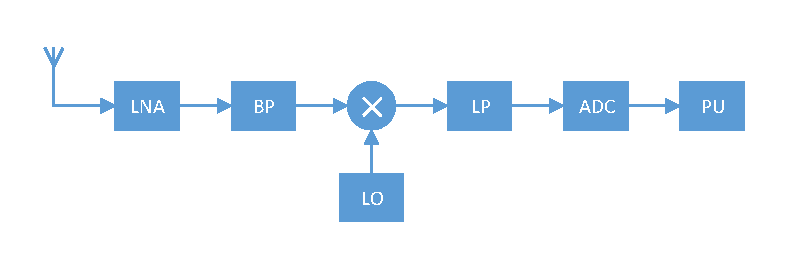
\includegraphics[width= \textwidth]{figures/Receiver.pdf}
\caption{A basic receiver structure.}
\label{fig:basic_receiver_structure}
\end{figure}

Each block will analysed with focus on the properties that could influence measurements on the fading gain i.e. gain, noise, distortion etc.

\textbf{Antenna}\\
In a line-of-sight case the received power can be expressed as \citep[p. 86]{balanis}:
%\begin{equation}
%s(t) = \int_0^{2\pi} \! \int_0^\pi G_{ant}(\theta,\phi)\cdot s(\theta,\phi,t) \,\text{d}\phi \,\text{d}\theta
%\end{equation} 
%\begin{where}
%\va{$s(t)$}{is the received signal at the antenna}{W}
%\va{$s(\theta,\phi,t)$}{is the signal strength in the $(\theta,\phi)$ direction}{W}
%\va{$G_{ant}(\theta,\phi)$}{is the gain in the $(\theta,\phi)$ direction}{1}
%\va{$\theta$}{is the azimuth angle}{rad}
%\va{$\phi$}{is the elevation}{rad}
%\end{where}

\begin{equation}
P_r(t) = \frac{D_t\cdot A_r}{4\pi\cdot R^2}\cdot P_t(t)
\end{equation} 
\begin{where}
\va{$P_r(t)$}{is the received signal at the receiving antenna}{W}
\va{$D_t$}{is the directivity of the transmitter antenna}{1}
\va{$A_r$}{is the effective area of the receiving antenna}{$m^2$}
\va{$R$}{is the distance between transmitter and receiver}{m}
\va{$P_t(t)$}{is the transmitted signal at the transmit antenna}{W}
\end{where}

It might be possible to use this to gain a extra dimension in the measurement setup, however it might also be a problem as the assumptions for the Doppler spectrum and often relies on omnidirectional reception. Normally it is possible to calibrate the system to account for gain to find the actual signal level, however it is not possible to account for an imbalance in the antenna pattern. 


Impedance mismatch typically occur where the signal is fed from the antenna to the rest of the system, this can be formulated as \citep[p. 63]{balanis}:

\begin{align}
%x_V(t) = (1+\Gamma)\cdot s_V(t) \\
%x_I(t) = (1-\Gamma)\cdot s_I(t) \\
x_P(t) = (1-|\Gamma|^2)\cdot P_r(t) \label{eq:ref_power}
\end{align}
\begin{where}
\va{$x_P(t)$}{is the power transmitted through to the system}{W}
\va{$\Gamma$}{is the reflection coefficient}{1}
\end{where}

This typically introduces both a gain and a phase distortion, however with calibration this is not an issue.

\textbf{\Gls{LNA}}\\
When the signal is passed through the LNA it can be described as:

\begin{equation}
x_{LNA}(t) = G_{LNA}\left(x_P(t)\right)*x_P(t)
\end{equation}
\begin{where}
\va{$x_{LNA}(t)$}{is the outputed signal from the LNA}{W}
\va{$G_{LNA}\left(x_P(t)\right)$}{is the gain of the LNA dependent on the input power}{1}
\end{where}

If the signal conforms to $|x_P(t)| < sat$ where sat is the saturation limit of the LNA, $G_{LNA}\left(x_P(t)\right)$ becomes a constant and the convolution becomes a multiplication, however if the power level reaches the saturation level then this is not the case and the complicated convolution is necessary. It is further not easy to calibrate for the distortion introduced by saturating the LNA.


\textbf{\Gls{BP}}\\
When the siganl is passed through a BP filter it can be described as
\begin{equation}
%x_{BP}(t) = H_{BP}(t)*\left(G_{LNA}\left(x_P(t)\right)*x_P(t)\right)
x_{BP}(t) = H_{BP}(t)*x_{LNA}(t)
\end{equation}
\begin{where}
\va{$x_{BP}(t)$}{is the signal outputted from the BP filter}{W}
\va{$H_{BP}(t)$}{is the impulse response of the BP filter}{1}
\end{where}

Implications of the BP is the signal becomes band limited which helps reduce noise, however for the filter to work it needs to settle and it also introduces a group delay. The settle time is often between $\frac{1}{f_c}$ and $\frac{3}{f_c}$%http://www.freqdev.com/guide/analog.html
but is highly dependent on the actual order of the filter. The group delay is however not easy to correct, it is therefore desirable to a linear phase shift through the filter as that introduces a constant delay to all frequencies, however in practice this is not case. 


\textbf{Mixer}\\
The mixer is the the only component that relies on its non-linearities in the chain. It takes two input namely the data caring signal and the mixing signal from the \gls{LO} a it can be modelled as \citep[p. 12]{Mixer}:
\begin{equation}
%x_{Mixer}(t) = \left(H_{BP}(t)*\left(G_{LNA}\left(x_P(t)\right)*x_P(t)\right)\right)\cdot sin\left(2\pi\cdot (f_{LO}+\epsilon_{drift}(t)) \cdot t\right)
x_{Mixer}(t) = x_{BP}(t) \cdot sin\left(2\pi\cdot (f_{LO}+\epsilon_{drift}(t)) \cdot t\right)
\end{equation}
\begin{where}
\va{$x_{Mixer}(t)$}{is the output from the mixer}{W}
\va{$f_{LO}$}{is the frequency of the LO}{Hz}
\va{$\epsilon_{drift}(t)$}{is the drift in frequency of the LO}{Hz}
\end{where}


Most of the distortion in the processed signal comes from this component, as the process is highly non-linear. The $\epsilon_{drift}(t)$ is often quite small and as long as it does not change the signal to conflict with the LP then it can typically be neglected for all intents and purposes. However a lot of extra frequency components is added to the signal due to the nature of the mixer.

%%%%%%%%%%%%%%%%%%%%%%%%%%%%%%%%%%%%%%
%%%%%%%%%%%%%%%%%%%%%%%%%%%%%%%%%%%%%%
% DO STUFF WITH THIS

%A filter needs approximately $\frac{1}{2\cdot fd_{max}}$\todo{find source (right now found from patricks mail} seconds to settle. This means a measurement should run for at least that amount of time, also the saturation can be avoided by lowering the transmit power. The frequency drift of a oscillator is typically $\pm 50ppm$ \todo{source, link is here} %$http://dk.farnell.com/webapp/wcs/stores/servlet/Search?catalogId=15001&langId=45&storeId=10157&categoryId=700000058502&pageSize=25&showResults=true$}

%%%%%%%%%%%%%%%%%%%%%%%%%%%%%%%%%%%%%%
%%%%%%%%%%%%%%%%%%%%%%%%%%%%%%%%%%%%%%

\textbf{\Gls{LP}}\\
The LP filter make sure that most of the unwanted components introduced from the mixer gets reduced significantly. It is modelled in much the same manner as the BP filter and comes with the same problems. 
\begin{equation}
%x_{LP}(t) = H_{LP}(t)*\left(\left(H_{BP}(t)*\left(G_{LNA}\left(x_P(t)\right)*x_P(t)\right)\right)\cdot \left(f_{LO}+\epsilon_{drift}(t)\right)\right)
x_{LP}(t) = H_{LP}(t)*x_{Mixer}
\end{equation}
\begin{where}
\va{$x_{LP}(t)$}{is the outputted from the LP filter}{W}
\va{$H_{LP}(t)$}{is the impulse response of the LP filter}{1}
\end{where}

The settle time of the LP is often magnitudes longer than the settle time of the BP as the frequencies involved are much lower. 

After this the \gls{ADC} quantise and digitalize the signal so a \gls{PU} can process it. Through this analysis different parameters have been found to affect the signal in the receiver, ending in a rather complicated expression. If an network analyser is used for measurement then most of these problems is dealt with, in a way that makes it of little concern e.g. the signal never saturates the amplifiers the drift in the LO is measured and accounted for etc. The rest of the distortion introduced can be calibrated as it is deterministic. 


%
%
%
%%These problems can be categorized into what can be accounted for during the measurement, what can be accounted for by calibrating the equipment and what can not be easily dealt with.
%%
%\begin{itemize}
%\item Avoidable problems
%	\begin{itemize}
%	\item Settle time
%	\item Saturation
%	\end{itemize}
%\item Calibration problems
%	\begin{itemize}
%	\item Reflection
%	\item Gains
%	\end{itemize}
%\item Distortion problems
%	\begin{itemize}	
%	\item Phase shift/ group delay
%	\item Drift
%	\item Non-linearities
%	%\item Effective number of bits
%	\end{itemize}
%%\item Statistical problems
%%	\begin{itemize}
%%	\item Noise
%%	\item Quantization noise
%%	\end{itemize}
%\end{itemize}
%%
%Parameters that is critical to the measurements is the BW and the antenna pattern as these two directly influence the measurement of the channel. The rest only has indirect implications on the measurements. This is supported by related work in \citep{MeasurementComplexRay}
\textbf{Noise}\\
A problem that has not been addressed is the noise aspect, all components in the receiver chain produces noise. Normally the figure of interest is the noise power a typical model for the noise power is a Gaussian process. As this process is a random process the noise can not be accounted for by calibration as with the distortion. Furthermore the Rayleigh fading model is a complex Gaussian process which means that it can be next to impossible to distinguish between the contribution from fading and noise in the received signal. Based on these arguments it is assumed that noise is the dominant factor which needs to be accounted for where the distortion introduced by the components will be less and in most cases reduced further by calibration.


\section{Dynamic range}
Dynamic range in RF systems is the ability of the receiver to pick out weak signals compared to the strong ones(the range of the low signals to the high signals which the receiver can operate). Think about it as trying to hear a person talking when somebody in the room is screaming.  
With manual or automatic gain control,the total dynamic range of the receiver will allow it to accept a wider range of signal power.That isn't a problem as long as we want to observe the strongest signal or nearly the strongest one.The situation gets tricky when we want to observe a really weak signal in the presence of much stronger ones.That is the point where we are more interested in the instantaneous dynamic range.
The instantaneous dynamic range is specified as the difference between the strongest to the weakest signal(in dB) that can be present in a receiver's pass band while the receiver is meeting full specified performance in receiving and processing the weaker signal.
The maximum strength that a receiving system can accept and process depends on the sensitivity of the receiver and it's dynamic range.
\begin{equation}
MAXstr_{dBm} = (Sens) +(DR)
\label{Max strength of a receiving system}
\end{equation}

Where $MAX_{str}$ is the maximum strength of a receiving system,Sens is the sensitivity of the receiver and DR the dynamic range of the system.\citep{DyR}

Receiver sensitivity is defined as the weakest signal that can be observed and still provide a sufficient quality output.Sensitivity is determined by the sum of Thermal Noise ,Noise Figure and the Required prediction of SNR.It is normally a negative number(in dBm) and this means that a bigger number(more negative) equals a smaller signal.
The thermal noise is given by:
\begin{equation}
Noise_{dBm} = 10log(BW\cdot Te\cdot k\cdot 1000) + NF
\label{Noise1}
\end{equation}
where $BW$ is the bandwidth $Te$ is the thermal temperature and the $NF$ is the noise figure of the reviver.

Dynamic Range or else Signal to noise and Distortion Ratio(SINAD) is also very similar to the Signal to Noise Ratio(SNR). SINAD is a good way to describe the whole dynamic system of ADC because takes into account all the components that make noise and distortion,in other words takes into account the non-linearities. The difference between them can be shown in high frequencies because the SINAD gets affected by the distortions and degrades faster than the SNR that excludes the first 5 harmonics that are dominant.The clear difference can be shown from the two formulas:
\begin{equation}
\text{SINAD} = 20log\left(\frac{S}{N+D}\right)
\end{equation}

\begin{equation}
\text{SNR} = 20log\left(\frac{S}{N}\right)
\end{equation}
where S represents the signal power,N the Noise and D the Distortion.\citep{SINADandSNR}
\subsection{SNR margin estimation}
\label{SNR_margin}
Because the noise might influence the deep fades of our signal, a minimum SNR margin needs to be estimated.
This gives us the SNR margin needed to distinguish a deep fade from the noise floor. % given a set confidence interval and margin.
%By doing this gives we will be able to accept the measurements that are above this margin and reject the ones that are affected by the noise.
The estimation assume the signal as a constant and the noise as a complex vector that changes. Therefore a Rician distribution can be used, because it consists of constant part and random part.
\begin{equation}
p = a^2 + 2\sigma^2
\end{equation}
\todo {change symbols}
Rician distribution fits in this situation because the K-factor that it depend upon is a ratio of power for the constant signal to the random noise, \citep{SpaceWirelessChan} meaning that the K-factor matches the SNR margin that we need to estimate.
\begin{equation}
K = \frac{a^2}{2\sigma^2}
\end{equation}
Given that we set our confidence interval of $\pm 1$dB around the value of our constant signal in the Rician cdf matched with the 90\% confidence level on the probability axis, we are able to estimate numerically the part of the K-factor that we are interested in.
\begin{figure}[H]
\centering
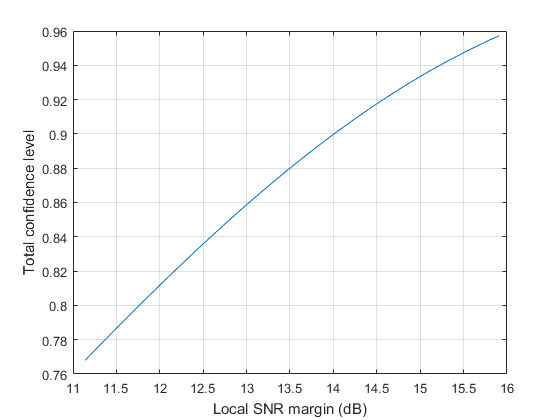
\includegraphics[width=0.70\textwidth]{figures/SNR_margin.png}
\caption{Solving for the K-factor numerical gives a estimate of SNR Margin. At 0.90 confidence with $\pm 1$dB margin  the K-factor is 14dB.}
\label{Rician_90}
\end{figure}

The results show that a SNR margin $SNR_m$ of 14dB is needed to have accurate reading of the deep fades.
The total dynamic range requirement becomes:
\begin{equation}
DR_{tot} = SNR_m - G_f , 14dB + 50dB = 64dB 
\end{equation}
\begin{where}
\va{$DR_{tot}$}{Total dynamic range}{dB}
\va{$SNR_m$}{is the SNR margin }{dB}
\va{$G_f$}{is the fading gain we want to measure (-50dB)}{dB}
\end{where}



\subsection{How to measure dynamic range}

In a normal receiver the dynamic range is set by the sensitivity of the receiver to the Third order intercept point. Third order intercept points are caused by over driving the receiver with too much input and that causes distortion and signal saturation. The sensitivity is more dependent on the operating environment and the receivers noise figure. \citep{understandDynamic}


\begin{figure}[H]
\centering
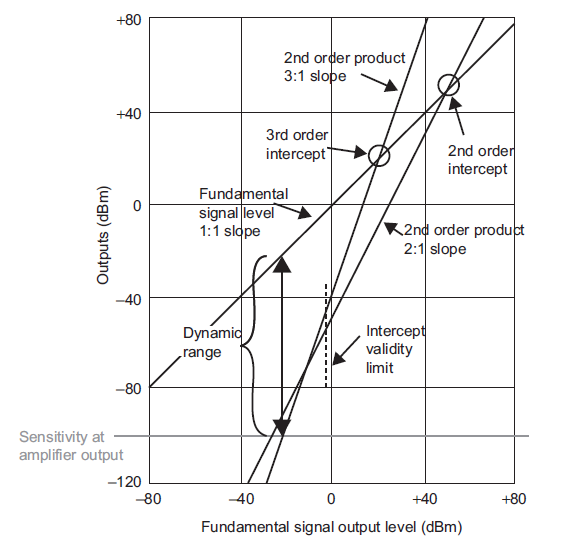
\includegraphics[width=0.90\textwidth]{figures/Dynamic_range_calc.png}
\caption{Determining the Dynamic Range from the spurs and sensitivity line.(WORK IN PROGRESS!!)}
\label{Dynamic_range_calc}
\end{figure}
To calculate the dynamic range we are interested on the third order products.The second order products they get filtered out due to the big distance from the original frequencies.When we have the third order products we draw a vertical line from the intercept point of the sensitivity and the third order products till the fundamental signal. This distance between the two lines defines the strength of the strong output signals that will cause distortion at the sensitivity level. In our example below the intercept point of the third order products and the sensitivity level is at -100dB while the vertical line meets the fundamental signal at -32dB meaning that the dynamic range is 68dB. 
%This means that a RF receiver is highly dependent on the mixer and amplifier with regards to dynamic range. A measurement system would take into account the factors listed in \autoref{basic_rev_struct} to increase the dynamic range. Going through the \autoref{fig:basic_receiver_structure} in order from left to right. The receivers \gls{IF} is the frequency that shifted to in order to process the signal easier.  This is done in the first stages of a receiver. This frequency is normally lower than the transmitted RF frequency, this especially helps the \gls{ADC} that uses a lower sampling rate. By setting the \gls{IF} filter to a very narrow bandwidth (narrowband) the noise floor goes down and increases the dynamic range. 

\section{Time to do a sweep}
The cost of using a narrowband is the measurement time, as the system would require a longer time for the sweep to cover a typical bandwidth. The time this would take is given by:
\todo{maybe write about averaging here and add it to the Time calculations}
\begin{equation}
T = \frac{1}{IF_{BW}} \cdot \frac{BW_{sweep}}{IF_{BW}}
\end{equation}
where $IF_{BW}$ is the intermediate frequency bandwidth and $BW_{sweep}$ is the total bandwidth you want to measure.


\subsection{Dynamic range in a VNA receiver}
\begin{figure}[H]
\centering
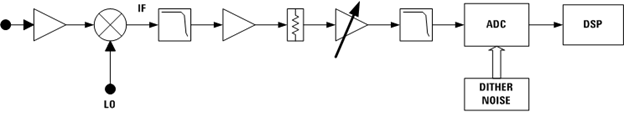
\includegraphics[width=0.90\textwidth]{figures/Block_VNA.png}
\caption{A Typical block diagram of a VNA receiver.}
\label{Block_VNA}
\end{figure}

For Network analysers the dynamic range is the maximum signal power the receiver can measure minus the noise floor of the receiver. To achieve a higher dynamic range of \gls{VNA} it must be  in tuned-receiver mode (Narrowband).
If you reduce the bandwidth then the overall noise floor will go down, so it logical that it would have higher dynamic range. \citep{AgilentNVA} \\
%%The setup of the \gls{VNA} measuring would have to take into account some factors to increase the dynamic range and still have the accuracy. Going through the \ref{Block_VNA} in order from left to right.
%%The \gls{IF} is a frequency that shifted to in order to process the signal easier. This is done in the first stages of a receiver. This frequency is normally lower than the transmitted RF frequency, this especially helps the \gls{ADC} that uses a lower sampling rate. 
%%By setting the \gls{IF} filter to a very narrow bandwidth (narrowband) the noise floor goes down and increases the dynamic range. The cost of using a narrowband is the measurement time, as the \gls{VNA} would need several sweeps to cover a typical bandwidth. \\

Dynamic range and accuracy are affected by the non-linearity in the receiver chain, the worst part are the mixers,\gls{ADC} and amplifiers since they introduce the most non-linearity. To measure the linearity of a receiver a power change measurements is preformed and compared to a reference level of power change that is accurate. This means that the linearity of a receiver as can be defined as:
\begin{equation}
Linearity = \frac{receiver \\\ measured \\\ power \\\ change}{reference \ power \ change}
\label{Linearity}
\end{equation}
 

Cross talk is the energy leakage between signal paths of the measuring system and it can be a problem in high-loss transmission measurements. This can be fixed by running an isolation calibration \citep{crosstalk}.It occurs below the noise floor so averaging and low \gls{IF} filter bandwidth must be used during calibration.
At low power levels <-70dBm the main non-linearity comes from the \gls{ADC}. Quantizing error occurs when converting from analog to digital signals. The \gls{ADC} used in \gls{VNA} are top of the line and can use a Gaussian noise ditcher to combat the non linear nature of a \gls{ADC}. 


In the digital signal processing of the \gls{VNA} averaging be applied to reduce the noise.Given the noise is uncorrelated, by averaging the measured(complex) data the noise component will approach zero.That means that our end signal in the output will be with less noise.Every time that our average is getting doubled, the signal to noise ratio is increased by 3dB. The problem is that by averaging the double of every data point the measurement will take twice as long.\citep{KeysightAVG}. The total noise floor is then given by:

\begin{equation}
Noisefloor_{dBm} = log_{2}(AVG_f)\cdot 3dB +10log(IF_{BW}\cdot T_{0}\cdot k\cdot 1000) + NF 
\label{NFwithAVG}
\end{equation}
Where $IF_{BW}$ is  intermediate bandwidth $T_0$ is temperature of the system, $k$ is the Boltzmann's constant,$AVG$ is the averaging factor and $NF$ if the noise figure.
To maximise the effectiveness of a \gls{VNA} the reviver $IF_{BW}$ should be high as possible for the dynamic range needed. So to get accurate samples with the needed dynamic range in the least amount of time the $IF_{BW}$ and $AVG_f$ must be balanced to minimise time spent on one measurement.
Equipment drift is another source of error that can occur if we are operating in a place with different environmental factors for a long period of time.


%\section{Diversity}
%% (effects?)
%Diversity is used to combat fading in a wireless system. By using clever techniques you can effectively deliver several copies or replicas of a signal to the receiver. There is a lower chance that all of these copies of signals are going to have a deep fade at the same time \citep[p. 4-6]{diversityFuture}. The overall goal is to provide a gain in signal quality by having several signals that independently fade from each other without the cost of more power consumption, reduced bit rate and complexity or other resources. There are several ways to achieve diversity in a wireless system. \\
%Time diversity: By retransmitting the same information you get some diversity gain on the cost of decreased bit/rate. Usually a forward error correction code is added instead of just re transmitting the signals several times. \\
%Antenna diversity / Spatial diversity
%By having several antennas at both/or the receiver and transmitter a antenna diversity is achieved. With several antennas the signal can be combined together to process the signals into one. To get independently fading signals the signals need to be uncorrelated by separating the antennas least half a wavelength (micro diversity) \citep{diversityAntenna}. Antenna diversity comes at the cost of having to power more than one antenna.


\subsection{How to measure uncorrelated samples}
\label{howtomeasureUS}
To measure the required samples from \autoref{sampleEQ} ($\approx 4.04\cdot10^6$) uncorrelated samples requires a elaborate test setup. The limitation is in how much space and time the measurement is going to require. The total number of samples that can be obtained can be expressed as: 
\todo {removed big part here, maybe move it to measurement setup}
%The example scenario  will have a $f_c$ of 3Ghz, BW of 100MHz, a $5x5$ antenna array, a office building with a delay spread of 100ns and a room size that is $10m \cdot 10m$.
%If we assume we have a multipath delay spread of 100ns. Given \autoref{CohBW} the $B_C$ is 1.6MHz. Since the $B_C$ is only a approximation with some coherence, the $B_C$ should be increased to approximate 3 Mhz to get less correlated samples. This will give round 30 uncorrelated samples in frequency with a BW of 100MHz.
%The $f_c$ of 3Ghz gives a $\lambda$ of 0.1m or 10cm. The array antennas has each antenna spaced half a $\lambda$ which would give a total antenna length of 0.25m. If the antenna array is moved in one dimension,every step needs to be spaced $0.25+\frac{\lambda}{2}$ apart. Given the 10m size of the room 30 samples is possible in 1 dimension. If the measurements is done in 2 dimensions ($10m\cdot 10m$) a total area of:

\begin{equation}
N = \underbrace{A_{div}}_\text{$N_a$} \cdot \underbrace{\frac{BW}{B_c \cdot 2}}_\text{$N_f$} \cdot \underbrace{\frac{\Delta}{(\frac{\lambda}{2})^2}}_\text{$N_d$}
\label{howtosample}
\end{equation} 
 
\begin{where}
\va{$N$}{Total samples}{1}
\va{$N_a$}{parallel antenna samples}{1}
\va{$N_f$}{samples in frequency}{1}
\va{$N_d$}{samples in space}{1}
\va{$A_{div}$}{antenna diversity}{1}
\va{$\Delta$}{is the area }{$m^2$}
\va{$B_c$}{is the coherence BW }{Hz}
\va{$\lambda$}{wavelength}{m}
\end{where} 
 
%Where $N$ is number of samples(in antenna diversity,frequency and space), $A_{div}$ is the antenna diversity, $\Delta$ is the area, $B_c$ is the coherence BW and $\lambda$ is the wavelength.

\autoref{howtosample} can be used to found the area required given number of samples $N$ needed.

\begin{equation}
\Delta  = \frac{N\cdot (\frac{\lambda}{2})^2}{A_{div}\cdot \frac{BW}{B_c \cdot 2}}
\label{howtosqaure}
\end{equation}

If the area of the measurement is not big enough to take all the measurements different rooms could be used. To do this you need to normalize for the mean gain the system sees. It's clear that taking $4.04\cdot10^6$  uncorrelated samples requires taking advantage of  frequency(bandwidth),space or time to get the necessary samples. The best way is to balance and connect these values to the limitation in the equipment and measurement setup. This will be examined in later sections. 
%If we assume a $10m \cdot 10m$ this gives us: 
%\begin{equation}
%\frac{10m}{\frac{\lambda}{2}} \cdot \frac{10m}{\frac{\lambda}{2}}  = 40000 samples
%\end{equation}
%The total amount of spatial, frequency and antenna array uncorrelated samples is:
%\begin{equation}
%30 \cdot 25 \cdot 40000 = 3 \cdot 10^7 samples
%\end{equation}
%which is way more then we need.
%Actually moving the reviver $2 \cdot 10^6$ times takes way to long to actually do, but this example calculation is just to show that it is possible to obtain $10^7$ samples.If the area of the measurement is not big enough to take all the measurements different rooms could be used. To do this you need to normalize for the mean gain the system sees. 

A other problem with a taking $4.04\cdot10^6$  uncorrelated samples is that the channel may be changing because of frequency shift or movement. This will make the samples uncorrelated, but you are in danger of measuring a completely different channel. Here comes the non-stationary principle into play. A argument could be made that the $10^{-5}$ fading is so dependant on the environment that a measurement would only be valid for this exact room or situation you are measuring.

\subsection{Time required to do measurements}
\todo{Write more general or remove/move to part II}
When trying to obtain a high number of samples, time becomes a very limiting factor. For this reason a estimation of total measurement time or a time budget is helpful. If one sample takes 1 second to measure and the required samples size is $10^7$, the total measuring time would be 116 days of continues measurements. This of course is not practical to do. So it's obvious that a automatic systems that takes several samples in parallel is needed. The time budget uses the values from  \autoref{howtomeasureUS} and assumes the samples are measured continuously in one dimension with a velocity of $1m/s$. 
The antenna array is spaced in a different dimension so samples don't overlap. The time it would take to do a $100MHz$ sweep is dependant on the $IF_{BW}$ and dynamic range requirements discussed later. The calculation assumes that system can do a full sweep over the BW at every $\frac{\lambda}{2} = 0.05m$ and get the 30 samples in frequency or $N_f$. So first lets calculate the amount of samples we can do per second $N_s$:
\begin{equation}
N_s = \frac{v}{\frac{\lambda}{2}}\cdot N_f \cdot A_{div}, \frac{1m/s}{0.05m} \cdot 30N \cdot 25N = 15000N_s
\end{equation}
Then the total time needed for a continues measurements:
\begin{equation}
T = \frac{N}{N_s} , \frac{10^7N}{15000N_s} = 667s \approx 12 minutes.
\end{equation}
The total time budget shows that multiple uncorrelated samples must be acquired at a relative high speed in order to get the needed sample size. A speed of $1m/s$ over 12 minutes is equal to $720m$ in one dimensions so a two dimensional space separation is needed to reduce the room size requirement.. The practicality of this will be discussed in part II.
%\section{Introduction of noisy signal}

\chapter{Statistics}

\section{Brute force}

First an estimate for the number of samples needed to achieve different confidence level and intervals is investigated. The number of samples needed is found using the normal approximation of the Binomial proportion \citep{SampleNumURC}. 

\begin{equation}
\frac{z_{\frac{\alpha}{2}} \sqrt{\hat{\gamma}\left(1-\hat{\gamma}\right)/N}}{\hat{\gamma}} < m
\end{equation} 
\begin{where}
\va{$z_{\frac{\alpha}{2}}$}{is the $100(1-\frac{\alpha}{2})$-th percentile of the standard normal distribution}{1}
\va{$\hat{\gamma}$}{is the estimated probability}{1}
\va{N}{is the number of samples}{1}
\va{m}{is the margin around $\hat{\gamma}$}{1}
\end{where}

% Please add the following required packages to your document preamble:
% \usepackage{multirow}
\begin{table}[H]
\centering
\begin{tabular}{c|l|l|l|l|l|l|}
\multicolumn{2}{l}{}  & \multicolumn{5}{c}{\textbf{Confidence level}} \\ \cline{3-7} 
\multicolumn{2}{l|}{}  & \textbf{80 \%} & \textbf{85 \%} & \textbf{90 \%} & \textbf{95 \%} & \textbf{99 \%} \\ \cline{2-7} 
\multirow{5}{*}{\rotatebox{90}{\textbf{Confidence interval}}} & \textbf{$\pm$0.5 dB} & 11.0E+6 & 13.9E+6 & 18.2E+6 & 25.8E+6 & 44.6E+6 \\ \cline{2-7} 
 & \textbf{$\pm$1 dB} 	& 2.45E+6 	& 3.09E+6 	& 4.04E+6 	& 5.73E+6 	& 9.90E+6 \\ \cline{2-7} 
 & \textbf{$\pm$1.5 dB} & 965E+3 	& 1.22E+6 	& 1.59E+6 	& 2.26E+6 	& 3.90E+6 \\ \cline{2-7} 
 & \textbf{$\pm$2 dB} 	& 480E+3 	& 606E+3 	& 791E+3 	& 1.12E+6 	& 1.94E+6 \\ \cline{2-7} 
 & \textbf{$\pm$2.5 dB} & 271E+3 	& 342E+3 	& 447E+3 	& 634E+3 	& 1.10E+6 \\ \cline{2-7} 
\end{tabular}
\caption{My caption}
\label{my-label}
\end{table}

\subsection{Statistical relations}


Confidence interval at $1-\alpha$ level:
\begin{equation}\label{interval}
\bar{x} \pm z_{\frac{\alpha}{2}} \cdot \sqrt{\frac{var(x)}{N}}
\end{equation}

Based on \autoref{interval} assuming a interval threshold, A
\begin{equation}\label{interval2}
N \geq \left(z_{\frac{\alpha}{2}} \cdot \frac{\sqrt{var(x)}}{A} \right)^2
\end{equation}

Using the normal approximation of the binomial proportion we  estimate the number of samples with 90\% confidence level and an interval threshold of $\pm 25\%$ or 1 dB.Based on the Equation 1.12 we have for $ \bar{x} = 10^{-5} $ :
\begin{equation}\label{sampleEQ}
N=(1.645)^{2} \cdot \frac{1}{(0.25)^{2}} \cdot \frac{1-\bar{x}}{\bar{x}} = 4.3 \cdot 10^{6}
\end{equation}
Because the above procedure is an approximation we would generate $ 10 \cdot 10^{6} $ number of samples.\citep{SampleNumURC}
\subsection{Limitation for measurement purposes}

Strict limitations
\begin{equation}
SNRs > 1
\end{equation}

Other limitations
\begin{equation}
E\left(SNR\right) \;>\, \frac{1}{raylinv(p,\theta)} 
\end{equation}

\begin{where}
\va{$x$}{is the individual sample}{NA}
\va{$xs$}{is a threshold value for the samples}{NA}
\va{$\theta$}{is the mode of the distribution}{NA}
\va{$SNRs$}{is the threshold value of the signal-to-noise ratio}{1}
\va{$SNR$}{is the individual sample of the signal-to-noise ratio}{1}
\va{$N$}{number of samples}{1}
\va{$z_{\frac{\alpha}{2}}$}{is the normalize interval from a standard distribution}{NA}
\end{where}



\section{Statistics method for rare events}
As seen in previous chapters, there is a need of a high number of samples, to get a high confidence interval. The reason for this, is there is a need of a high number of rare events to occur to get a high confidence interval for this events. 

For simulations there have been developed some methods to handle this problem. One of them is importance sampling. Importance sampling changes the distribution where the samples is taken from. By changing the distribution, so the rare events is not rare anymore and a high number of them can be samples with a smaller sample population. When introduction this new distribution, there also needs to be introduced a weighting factor. This weighting factor is defined from the change in the different distribution. This weighting factor is used to go from the actually distribution to the new created distribution.

Most of the other methods used in simulation to handle this problem with rare events, changes the distribution, as this is one of the known parameters for simulations. A problem when using these methods, is that in the real world the exactly distribution is not known, so weighting factor, that is the difference between the real and new created distribution can only be a estimate. But these methods can not be used in the real world to reduce the number of samples needed needed for this measurement campaign, as the distribution in the real world would have to be force fulled changed, so the rare events will happen more often. To do that, more deep fade spots have to be introduced into the room used for measurements, which can be done. But the measurements will not be the true picture of the distribution, unless the weighting factor is calculated precise enough and the new distribution is known.



%Reduction of number of samples
%- Important sampling
%- Not useful

\section{Bootstrap}
Another statistically aspect, which there are different method and techniques for, is how to determent the confidence interval at a certain confidence level. From the previous calculation of the number of samples needed in section \todo{Missing ref to section}, there is used a confidence level of 90\% \todo{Check this}. This is attain from doing a high number of measurements. This high number of measurements will be very time consuming. Hence there can be look at on a statistically method to determent the confidence interval, by having a lower number of samples. One of these methods is bootstrap.

Bootstrap is a method, where one take a large amount of samples from big sample space. This surrogate population, as the measurements made up, will then be a estimate of true sample population. From this surrogate population a series of phantom samples are made. This is done with making a simulation, where there are used the same number of samples, as in the original measurements, where the samples are picked uniformly from the surrogate population. This process is done a few thousand times, where the wanted value wanted to measured can be put into a histogram, where normale usage of getting the confidence level can be used. As in case of a interval of 90\%, the upper and lower 5\% will be cut off and this will give the confidence interval.

This method will still need a high number of samples, as there is still needed for some rare events to occur. But the sample size do not need to be as large as seen in section \todo{More refs}. This comes from that there will instead be used computation power instead to generate these phantom samples, which replaces the many other real life sample. 

\todo{Need example. A example used an example of our project, but on $10^{-3}$ would be great i think}






%\subsection{Statistics modeling from measurements}
%Model/Regression (Maximum likely hood)
%- Usage of bootstraping to estimate the a's in regression
\part{Data acquisition}
\chapter{Measurement Campaign}
\section{Setup}
The setup of the measurement will give the insight and solutions to the problems hypothesised in previous chapters. 
\subsection{equipment}
\label{equip}
Keysight \gls{VNA} N5527A 

Antenna array 4Ghz $f_c$.


%The most important part of the setup is the equipment and how they are connected. The R\&S Spectrum Analyser (model FPL9KHz-6GHz) is the center of the setup. This is the receiver of our system and gives us a readout of the spectrum in terms of power (dBm) and frequency (Hz). The two main setting on the Spectrum analyser is IF filter bandwidth and resolution. These two values gives us a sweep time.
\subsection{Specifications}
In chapter 1 all the needed factors has been discussed. Now when the setup is designed it's important to set specifications.
\begin{table}[]
\centering
\caption{My caption}
\label{final_specs}
\begin{tabular}{|l|l|l|l|}
\hline
Number of samples needed         & N           & 4.04 million   & $4.04 10^6$        \\ \hline
Center Frequency                 & $f_c$       & 4Ghz           & $4 \cdot 10^9$     \\ \hline
Wavelength                       & $\lambda$   & 10cm           & 0.075m               \\ \hline
Coherence freq                   & $\Delta f$  & 3MHz           & $3 \cdot 10^6$     \\ \hline
Dynamic range                    & DR          & 104dB           & $2\cdot 10^10$             \\ \hline
Antenna diversity                & $A_{div}$   & 1x3            & 3                  \\ \hline
Intermediate frequency bandwidth & $IF_{BW}$     & 10KHz          & $10 \cdot 10^3$ \\ \hline
\end{tabular}
\end{table}
\subsection{Total Dynamic range}
Given \autoref{total_prx} and the VNA specification given in \autoref{equip} we can find the total received power seen in the measurements and calculate the total dynamic range needed given the margin in \autoref{SNR_margin}:
\begin{equation}
L = 20log (4000MHz) + 28 \cdot log(8)-28 = 69dB
\end{equation}
\begin{equation}
DR_{tot} = 69dB - 30dBm + 64dB = 104dB 
\end{equation}
\section{Results}
\chapter{Discussion}
The discussion will follow up on the results found in \autoref{ch:MassTest} and \autoref{ch:BatTest} and suggestions are made to explain some of the findings, as well as some of the potential problems that might influence the results. 

\section{Domain: Massiveness}


\section{Domain: Energy Consumption}
It was found in \autoref{ch:BatTest} that it is possible to achieve a battery lifetime of more than 10 years on a 5 Wh battery, however it was also discovered that this was not a guarantee. It was found that to achieve this the device is only allowed to transmit for a maximum of \todo{find value}{} per 24 hours. 

Taking a step back to evaluate the method of finding this value, a couple of issues can be seen. The way the model is designed limits the precision a bit, this comes in two parts first is that TX and RX can not be told apart. This is needed for a couple of different reasons to better the results, first is this could be used to approximate the energy spent during the attach and release procedures more accurately, second is it would give way better options for designing a use case including e.g. software updates. The model handles this issue by always assuming a worst case scenario energy consumption, this however leads to the second issue. During the transmit phase RX is included, this lowers the power average power used here, as the model does not assume any relation between $T_{transmit}$ and the throughput this is not a major issue, but is does not accurately describe most use cases. The third issue is a bit more hidden however, the parameter repetition was set to 1, this means that any transmission is rather short when this parameter is increase factors like the transmission gap comes into play this is not accounted for in the model. The forth issue is that the model uses a full attach procedure for each attach, this should not be the case in a real scenario, however as this issue makes the model underestimate the lifetime the design objective can still be evaluated.

Fixing these flaws in the model could indeed bring the accuracy of the model up, however it would also complicate the model further. As the model is intended to be as simple as possible while still providing accurate estimates this is not desired. To evaluate if the model actually predicts the battery life time accurately would require a longer test run, setting all the parameters and including idle mode and data transmission interval and evaluating the energy consumption over multiple days. This has however not been possible as the UXM used in the project is a shared resource. 

Another concern is that only four parameters was chosen out of a multitude of parameters, this of course could influence the estimate quite a bit. This has been accounted for indirectly as more or less all of these parameters would affect the time a transmission takes, but not the average power consumption. A concern however is that repetition not only affects the data transfer but also the attach, release and paging messages. A few other parameters might also affect these procedures, in an uncertain way.

When all of these issues and concerns are taking into account the model still predicts that the main influence the battery lifetime is the transmit time and in the end this parameter is very much use case dependent. Other parameters is also highly influential such as idle mode timer values, however the scenarios for which they are a problem is considered quite unrealistic. 

	
\chapter{Conclusion}

When designing a measurement campaign prerequisites are important. A large part of the project was understanding how channel behaviour and how this can be represented in a stochastic manner. These models needs to be justified and connected to real world multipath environment. The deep fades that needs to be addressed in \gls{URLLC} are not empirically tested for but assumed. (assumed not necessarily known)

A statistical method of estimating the number of samples needed to validate the measurement to a 90\% $\pm 1dB$ was found. To further decrease the required amount of samples, several statistical techniques where investigated. But no such technique can be used because it changes the overall distribution. However the bootstrap is a useful method that can provide the confidence level and margin with the given samples.

To investigate the deep fades that needs to be dealt with to deliver an connection that fulfils the \gls{URLLC} conditions, requires an extensive amount of samples. Therefore the spatial and temporal domains has to be taken advantage of. To achieve this optimal frequency and space separation needed to be estimated

To validate the measurement of these predicted deep fades a large dynamic range is required. Together with the large dynamic range a large amount of samples are needed. These two part are linked has to be balanced and adjusted to make a measurement possible to do. An SNR margin is also needed to confirm that it's the signal and not the noise being measured

The results presented shows that the wanted confidence level of 90\% with a $\pm 1dB$ margin was not achieved and it had to be increased to $\pm 1.33dB$.\todo{update numbers if needed}


%\textbf{General problem statement:}
%Design a measurement system that can handle very deep fades and a statistical method to process the data and compare to existing models used in URLLC channels.

%This can be further specified to a more technical problem statement: \todo{Where do these numbers come from and why do we have two statements just after each other?!?}

%Ascertain with 90\% confidence with a 1 dB (25\%) margin that in a multipath environment, the cumulative distribution function of the fading gain can be assumed to increase in a log log linear fashion between -50dB and -20dB.

%To this it is important to investigate the following points: 
%\begin{itemize}
%	\item Find connections between channel statistics and sample size.
%	\item Find the reasonable confidence interval based on the minimum required sample size.
%	\begin{itemize}
%	\item Look into if there is a way to reduce the amount of samples needed by using statistical techniques.
% 	\end{itemize}
%	\item Figure out how to obtain uncorrelated samples in space,time and frequency.
%	\item Balance the sample acquisition for available resources. 
%	\item Design  a measurement setup that can acquire the samples needed.
%	\item Specify a method to process the obtained channel measurements.
%	\item Analyse the measurement and link the results to the current assumptions.
%\end{itemize}





%% literaturliste og bilag %%
\bookmarksetup{startatroot}% this is it
\addtocontents{toc}{\bigskip}% perhaps as well
\bibliography{setup/mybib}
\label{bib:mybiblio}
 
 \newpage
 \fancyhead[RO]{\small Appendix \nouppercase\rightmark} %even page - chapter title
 \fancyhead[LE]{\small Appendix \nouppercase\rightmark} %uneven page - section title
\fancyhead[RE,LO]{}
 \titleformat{\section}[hang]{\Large\bfseries}{\thesection\hsp\textcolor{black}{|}\hsp}{0pt}{\Large\bfseries}

 \renewcommand{\thesection}{\Alph{section}}
 \setcounter{section}{0}




\chapter*{Appendix}
 \addcontentsline{toc}{chapter}{Appendix}
 \addtocounter{chapter}{1}




\end{document}